% Options for packages loaded elsewhere
\PassOptionsToPackage{unicode}{hyperref}
\PassOptionsToPackage{hyphens}{url}
%
\documentclass[
  ignorenonframetext,
]{beamer}
\usepackage{pgfpages}
\setbeamertemplate{caption}[numbered]
\setbeamertemplate{caption label separator}{: }
\setbeamercolor{caption name}{fg=normal text.fg}
\beamertemplatenavigationsymbolsempty
% Prevent slide breaks in the middle of a paragraph
\widowpenalties 1 10000
\raggedbottom
\setbeamertemplate{part page}{
  \centering
  \begin{beamercolorbox}[sep=16pt,center]{part title}
    \usebeamerfont{part title}\insertpart\par
  \end{beamercolorbox}
}
\setbeamertemplate{section page}{
  \centering
  \begin{beamercolorbox}[sep=12pt,center]{part title}
    \usebeamerfont{section title}\insertsection\par
  \end{beamercolorbox}
}
\setbeamertemplate{subsection page}{
  \centering
  \begin{beamercolorbox}[sep=8pt,center]{part title}
    \usebeamerfont{subsection title}\insertsubsection\par
  \end{beamercolorbox}
}
\AtBeginPart{
  \frame{\partpage}
}
\AtBeginSection{
  \ifbibliography
  \else
    \frame{\sectionpage}
  \fi
}
\AtBeginSubsection{
  \frame{\subsectionpage}
}
\usepackage{amsmath,amssymb}
\usepackage{iftex}
\ifPDFTeX
  \usepackage[T1]{fontenc}
  \usepackage[utf8]{inputenc}
  \usepackage{textcomp} % provide euro and other symbols
\else % if luatex or xetex
  \usepackage{unicode-math} % this also loads fontspec
  \defaultfontfeatures{Scale=MatchLowercase}
  \defaultfontfeatures[\rmfamily]{Ligatures=TeX,Scale=1}
\fi
\usepackage{lmodern}
\usetheme[]{Madrid}
\ifPDFTeX\else
  % xetex/luatex font selection
\fi
% Use upquote if available, for straight quotes in verbatim environments
\IfFileExists{upquote.sty}{\usepackage{upquote}}{}
\IfFileExists{microtype.sty}{% use microtype if available
  \usepackage[]{microtype}
  \UseMicrotypeSet[protrusion]{basicmath} % disable protrusion for tt fonts
}{}
\makeatletter
\@ifundefined{KOMAClassName}{% if non-KOMA class
  \IfFileExists{parskip.sty}{%
    \usepackage{parskip}
  }{% else
    \setlength{\parindent}{0pt}
    \setlength{\parskip}{6pt plus 2pt minus 1pt}}
}{% if KOMA class
  \KOMAoptions{parskip=half}}
\makeatother
\usepackage{xcolor}
\newif\ifbibliography
\usepackage{color}
\usepackage{fancyvrb}
\newcommand{\VerbBar}{|}
\newcommand{\VERB}{\Verb[commandchars=\\\{\}]}
\DefineVerbatimEnvironment{Highlighting}{Verbatim}{commandchars=\\\{\}}
% Add ',fontsize=\small' for more characters per line
\usepackage{framed}
\definecolor{shadecolor}{RGB}{248,248,248}
\newenvironment{Shaded}{\begin{snugshade}}{\end{snugshade}}
\newcommand{\AlertTok}[1]{\textcolor[rgb]{0.94,0.16,0.16}{#1}}
\newcommand{\AnnotationTok}[1]{\textcolor[rgb]{0.56,0.35,0.01}{\textbf{\textit{#1}}}}
\newcommand{\AttributeTok}[1]{\textcolor[rgb]{0.13,0.29,0.53}{#1}}
\newcommand{\BaseNTok}[1]{\textcolor[rgb]{0.00,0.00,0.81}{#1}}
\newcommand{\BuiltInTok}[1]{#1}
\newcommand{\CharTok}[1]{\textcolor[rgb]{0.31,0.60,0.02}{#1}}
\newcommand{\CommentTok}[1]{\textcolor[rgb]{0.56,0.35,0.01}{\textit{#1}}}
\newcommand{\CommentVarTok}[1]{\textcolor[rgb]{0.56,0.35,0.01}{\textbf{\textit{#1}}}}
\newcommand{\ConstantTok}[1]{\textcolor[rgb]{0.56,0.35,0.01}{#1}}
\newcommand{\ControlFlowTok}[1]{\textcolor[rgb]{0.13,0.29,0.53}{\textbf{#1}}}
\newcommand{\DataTypeTok}[1]{\textcolor[rgb]{0.13,0.29,0.53}{#1}}
\newcommand{\DecValTok}[1]{\textcolor[rgb]{0.00,0.00,0.81}{#1}}
\newcommand{\DocumentationTok}[1]{\textcolor[rgb]{0.56,0.35,0.01}{\textbf{\textit{#1}}}}
\newcommand{\ErrorTok}[1]{\textcolor[rgb]{0.64,0.00,0.00}{\textbf{#1}}}
\newcommand{\ExtensionTok}[1]{#1}
\newcommand{\FloatTok}[1]{\textcolor[rgb]{0.00,0.00,0.81}{#1}}
\newcommand{\FunctionTok}[1]{\textcolor[rgb]{0.13,0.29,0.53}{\textbf{#1}}}
\newcommand{\ImportTok}[1]{#1}
\newcommand{\InformationTok}[1]{\textcolor[rgb]{0.56,0.35,0.01}{\textbf{\textit{#1}}}}
\newcommand{\KeywordTok}[1]{\textcolor[rgb]{0.13,0.29,0.53}{\textbf{#1}}}
\newcommand{\NormalTok}[1]{#1}
\newcommand{\OperatorTok}[1]{\textcolor[rgb]{0.81,0.36,0.00}{\textbf{#1}}}
\newcommand{\OtherTok}[1]{\textcolor[rgb]{0.56,0.35,0.01}{#1}}
\newcommand{\PreprocessorTok}[1]{\textcolor[rgb]{0.56,0.35,0.01}{\textit{#1}}}
\newcommand{\RegionMarkerTok}[1]{#1}
\newcommand{\SpecialCharTok}[1]{\textcolor[rgb]{0.81,0.36,0.00}{\textbf{#1}}}
\newcommand{\SpecialStringTok}[1]{\textcolor[rgb]{0.31,0.60,0.02}{#1}}
\newcommand{\StringTok}[1]{\textcolor[rgb]{0.31,0.60,0.02}{#1}}
\newcommand{\VariableTok}[1]{\textcolor[rgb]{0.00,0.00,0.00}{#1}}
\newcommand{\VerbatimStringTok}[1]{\textcolor[rgb]{0.31,0.60,0.02}{#1}}
\newcommand{\WarningTok}[1]{\textcolor[rgb]{0.56,0.35,0.01}{\textbf{\textit{#1}}}}
\usepackage{graphicx}
\makeatletter
\def\maxwidth{\ifdim\Gin@nat@width>\linewidth\linewidth\else\Gin@nat@width\fi}
\def\maxheight{\ifdim\Gin@nat@height>\textheight\textheight\else\Gin@nat@height\fi}
\makeatother
% Scale images if necessary, so that they will not overflow the page
% margins by default, and it is still possible to overwrite the defaults
% using explicit options in \includegraphics[width, height, ...]{}
\setkeys{Gin}{width=\maxwidth,height=\maxheight,keepaspectratio}
% Set default figure placement to htbp
\makeatletter
\def\fps@figure{htbp}
\makeatother
\setlength{\emergencystretch}{3em} % prevent overfull lines
\providecommand{\tightlist}{%
  \setlength{\itemsep}{0pt}\setlength{\parskip}{0pt}}
\setcounter{secnumdepth}{-\maxdimen} % remove section numbering
\logo{
\includegraphics[height=1cm,width=3cm]{logo.png}}
\usetheme{Madrid}
\usefonttheme{serif}
\setbeamertemplate{navigation symbols}{}
\usepackage{lmodern}  % for bold teletype font
\usepackage{amsmath}  % for \hookrightarrow
\usepackage{xcolor}   % for \textcolor


\ifLuaTeX
  \usepackage{selnolig}  % disable illegal ligatures
\fi
\usepackage{bookmark}
\IfFileExists{xurl.sty}{\usepackage{xurl}}{} % add URL line breaks if available
\urlstyle{same}
\hypersetup{
  pdftitle={Leksioni 13},
  pdfauthor={Endri Raco},
  hidelinks,
  pdfcreator={LaTeX via pandoc}}

\title{Leksioni 13}
\author{Endri Raco}
\date{04 July, 2024}

\begin{document}
\frame{\titlepage}

\begin{frame}[allowframebreaks]
  \tableofcontents[hideallsubsections]
\end{frame}
\section{}\label{section}

\begin{frame}[fragile]{Fillojmë me një tabelë}
\phantomsection\label{fillojmuxeb-me-njuxeb-tabeluxeb}
\AddToHookNext{env/Highlighting/begin}{\tiny}

\begin{Shaded}
\begin{Highlighting}[]
\CommentTok{{-}{-} Krijo tabelën Klientë}
\KeywordTok{CREATE} \KeywordTok{TABLE}\NormalTok{ Klientë (}
\NormalTok{  idKlienti }\DataTypeTok{int} \KeywordTok{PRIMARY} \KeywordTok{KEY}\NormalTok{ IDENTITY(}\DecValTok{1}\NormalTok{,}\DecValTok{1}\NormalTok{),}
\NormalTok{  emri }\DataTypeTok{varchar}\NormalTok{(}\DecValTok{50}\NormalTok{),}
\NormalTok{  mbiemri }\DataTypeTok{varchar}\NormalTok{(}\DecValTok{50}\NormalTok{),}
\NormalTok{  email }\DataTypeTok{varchar}\NormalTok{(}\DecValTok{100}\NormalTok{) }\KeywordTok{UNIQUE}\NormalTok{,}
\NormalTok{  telefoni }\DataTypeTok{varchar}\NormalTok{(}\DecValTok{20}\NormalTok{),}
\NormalTok{  adresa }\DataTypeTok{varchar}\NormalTok{(}\DecValTok{255}\NormalTok{),}
\NormalTok{  qyteti }\DataTypeTok{varchar}\NormalTok{(}\DecValTok{50}\NormalTok{),}
\NormalTok{  shteti }\DataTypeTok{varchar}\NormalTok{(}\DecValTok{50}\NormalTok{),}
\NormalTok{  kodi\_postar }\DataTypeTok{varchar}\NormalTok{(}\DecValTok{10}\NormalTok{),}
\NormalTok{  data\_regjistrimit }\DataTypeTok{DATE} \KeywordTok{DEFAULT}\NormalTok{ GETDATE()}
\NormalTok{);}
\end{Highlighting}
\end{Shaded}
\end{frame}

\begin{frame}[fragile]{Fillojmë me një tabelë}
\phantomsection\label{fillojmuxeb-me-njuxeb-tabeluxeb-1}
\AddToHookNext{env/Highlighting/begin}{\tiny}

\begin{Shaded}
\begin{Highlighting}[]
\CommentTok{{-}{-} Mbush tabelën Klientë me të dhëna shembull}
\KeywordTok{INSERT} \KeywordTok{INTO}\NormalTok{ Klientë (emri, mbiemri, email, telefoni, adresa, qyteti, shteti, kodi\_postar)}
\KeywordTok{VALUES}\NormalTok{ (}\StringTok{\textquotesingle{}Ana\textquotesingle{}}\NormalTok{, }\StringTok{\textquotesingle{}Hoxha\textquotesingle{}}\NormalTok{, }\StringTok{\textquotesingle{}ana.hoxha@example.com\textquotesingle{}}\NormalTok{, }\StringTok{\textquotesingle{}0681234567\textquotesingle{}}\NormalTok{, }\StringTok{\textquotesingle{}Rruga e Dibrës 12\textquotesingle{}}\NormalTok{, }\StringTok{\textquotesingle{}Tiranë\textquotesingle{}}\NormalTok{, }\StringTok{\textquotesingle{}Shqipëri\textquotesingle{}}\NormalTok{, }\StringTok{\textquotesingle{}1001\textquotesingle{}}\NormalTok{);}

\KeywordTok{INSERT} \KeywordTok{INTO}\NormalTok{ Klientë (emri, mbiemri, email, telefoni, adresa, qyteti, shteti, kodi\_postar)}
\KeywordTok{VALUES}\NormalTok{ (}\StringTok{\textquotesingle{}Maria\textquotesingle{}}\NormalTok{, }\StringTok{\textquotesingle{}Anders\textquotesingle{}}\NormalTok{, }\StringTok{\textquotesingle{}maria.anders@alfredsfutterkiste.com\textquotesingle{}}\NormalTok{, }\StringTok{\textquotesingle{}0123456789\textquotesingle{}}\NormalTok{, }\StringTok{\textquotesingle{}Obere Str. 57\textquotesingle{}}\NormalTok{, }\StringTok{\textquotesingle{}Berlin\textquotesingle{}}\NormalTok{, }\StringTok{\textquotesingle{}Germany\textquotesingle{}}\NormalTok{, }\StringTok{\textquotesingle{}12209\textquotesingle{}}\NormalTok{);}

\KeywordTok{INSERT} \KeywordTok{INTO}\NormalTok{ Klientë (emri, mbiemri, email, telefoni, adresa, qyteti, shteti, kodi\_postar)}
\KeywordTok{VALUES}\NormalTok{ (}\StringTok{\textquotesingle{}Ana\textquotesingle{}}\NormalTok{, }\StringTok{\textquotesingle{}Trujillo\textquotesingle{}}\NormalTok{, }\StringTok{\textquotesingle{}ana.trujillo@emparedadosyhelados.com\textquotesingle{}}\NormalTok{, }\StringTok{\textquotesingle{}9876543210\textquotesingle{}}\NormalTok{, }\StringTok{\textquotesingle{}Avda. de la Constitución 2222\textquotesingle{}}\NormalTok{, }\StringTok{\textquotesingle{}México D.F.\textquotesingle{}}\NormalTok{, }\StringTok{\textquotesingle{}Mexico\textquotesingle{}}\NormalTok{, }\StringTok{\textquotesingle{}05021\textquotesingle{}}\NormalTok{);}

\KeywordTok{INSERT} \KeywordTok{INTO}\NormalTok{ Klientë (emri, mbiemri, email, telefoni, adresa, qyteti, shteti, kodi\_postar)}
\KeywordTok{VALUES}\NormalTok{ (}\StringTok{\textquotesingle{}Antonio\textquotesingle{}}\NormalTok{, }\StringTok{\textquotesingle{}Moreno\textquotesingle{}}\NormalTok{, }\StringTok{\textquotesingle{}antonio.moreno@taqueria.com\textquotesingle{}}\NormalTok{, }\StringTok{\textquotesingle{}1234567890\textquotesingle{}}\NormalTok{, }\StringTok{\textquotesingle{}Mataderos 2312\textquotesingle{}}\NormalTok{, }\StringTok{\textquotesingle{}México D.F.\textquotesingle{}}\NormalTok{, }\StringTok{\textquotesingle{}Mexico\textquotesingle{}}\NormalTok{, }\StringTok{\textquotesingle{}05023\textquotesingle{}}\NormalTok{);}

\KeywordTok{INSERT} \KeywordTok{INTO}\NormalTok{ Klientë (emri, mbiemri, email, telefoni, adresa, qyteti, shteti, kodi\_postar)}
\KeywordTok{VALUES}\NormalTok{ (}\StringTok{\textquotesingle{}Thomas\textquotesingle{}}\NormalTok{, }\StringTok{\textquotesingle{}Hardy\textquotesingle{}}\NormalTok{, }\StringTok{\textquotesingle{}thomas.hardy@aroundthehorn.com\textquotesingle{}}\NormalTok{, }\StringTok{\textquotesingle{}2345678901\textquotesingle{}}\NormalTok{, }\StringTok{\textquotesingle{}120 Hanover Sq.\textquotesingle{}}\NormalTok{, }\StringTok{\textquotesingle{}London\textquotesingle{}}\NormalTok{, }\StringTok{\textquotesingle{}UK\textquotesingle{}}\NormalTok{, }\StringTok{\textquotesingle{}WA1 1DP\textquotesingle{}}\NormalTok{);}

\KeywordTok{INSERT} \KeywordTok{INTO}\NormalTok{ Klientë (emri, mbiemri, email, telefoni, adresa, qyteti, shteti, kodi\_postar)}
\KeywordTok{VALUES}\NormalTok{ (}\StringTok{\textquotesingle{}Christina\textquotesingle{}}\NormalTok{, }\StringTok{\textquotesingle{}Berglund\textquotesingle{}}\NormalTok{, }\StringTok{\textquotesingle{}christina.berglund@berglundssnabbkop.com\textquotesingle{}}\NormalTok{, }\StringTok{\textquotesingle{}3456789012\textquotesingle{}}\NormalTok{, }\StringTok{\textquotesingle{}Berguvsvägen 8\textquotesingle{}}\NormalTok{, }\StringTok{\textquotesingle{}Luleå\textquotesingle{}}\NormalTok{, }\StringTok{\textquotesingle{}Sweden\textquotesingle{}}\NormalTok{, }\StringTok{\textquotesingle{}S{-}958 22\textquotesingle{}}\NormalTok{);}

\KeywordTok{INSERT} \KeywordTok{INTO}\NormalTok{ Klientë (emri, mbiemri, email, telefoni, adresa, qyteti, shteti, kodi\_postar)}
\KeywordTok{VALUES}\NormalTok{ (}\StringTok{\textquotesingle{}Kardinali\textquotesingle{}}\NormalTok{, }\StringTok{\textquotesingle{}Tom B. Erichsen\textquotesingle{}}\NormalTok{, }\StringTok{\textquotesingle{}tom.kardinal@gmail.com\textquotesingle{}}\NormalTok{, }\StringTok{\textquotesingle{}454664446\textquotesingle{}}\NormalTok{, }\StringTok{\textquotesingle{}Skagen 21\textquotesingle{}}\NormalTok{, }\StringTok{\textquotesingle{}Stavanger\textquotesingle{}}\NormalTok{,}\StringTok{\textquotesingle{}Norvegji\textquotesingle{}}\NormalTok{, }\StringTok{\textquotesingle{}4006\textquotesingle{}}\NormalTok{);}
\end{Highlighting}
\end{Shaded}
\end{frame}

\begin{frame}{Deklarata INSERT INTO}
\phantomsection\label{deklarata-insert-into}
Deklarata INSERT INTO përdoret për të futur të dhëna të reja në një
tabelë.
\end{frame}

\begin{frame}[fragile]{Sintaksa INSERT INTO}
\phantomsection\label{sintaksa-insert-into}
\begin{itemize}
\item
  Është e mundur të shkruhet deklarata \textbf{INSERT INTO} në dy
  mënyra:

  \begin{enumerate}
  \tightlist
  \item
    Specifikoni emrat e kolonave dhe vlerat që do të futen:
  \end{enumerate}
\end{itemize}

\begin{Shaded}
\begin{Highlighting}[]
    \KeywordTok{INSERT}\NormalTok{ NË emrin e tabelës (kolona }\DecValTok{1}\NormalTok{, kolona }\DecValTok{2}\NormalTok{, kolona }\DecValTok{3}\NormalTok{, }\OperatorTok{..}\NormalTok{.)}
    \KeywordTok{VALUES}\NormalTok{ (vlera1, vlera2, vlera3, }\OperatorTok{..}\NormalTok{.);}
\end{Highlighting}
\end{Shaded}
\end{frame}

\begin{frame}{Sintaksa INSERT INTO}
\phantomsection\label{sintaksa-insert-into-1}
\begin{enumerate}
\setcounter{enumi}{1}
\tightlist
\item
  Nëse po shtoni vlera për të gjitha kolonat e tabelës, nuk keni nevojë
  të specifikoni emrat e kolonave në query-n SQL.
\end{enumerate}

\begin{itemize}
\tightlist
\item
  Megjithatë, sigurohuni që rendi i vlerave të jetë në të njëjtin rend
  si kolonat në tabelë.
\end{itemize}
\end{frame}

\begin{frame}[fragile]{Sintaksa INSERT INTO}
\phantomsection\label{sintaksa-insert-into-2}
\begin{itemize}
\tightlist
\item
  Këtu, sintaksa \textbf{INSERT INTO} do të ishte si më poshtë:
\end{itemize}

\begin{Shaded}
\begin{Highlighting}[]
  \KeywordTok{INSERT} \KeywordTok{INTO}\NormalTok{ table\_name}
  \KeywordTok{VALUES}\NormalTok{ (vlera1, vlera2, vlera3, }\OperatorTok{..}\NormalTok{.);}
\end{Highlighting}
\end{Shaded}
\end{frame}

\begin{frame}{Shembull}
\phantomsection\label{shembull}
Deklarata e mëposhtme SQL fut një rekord të ri në tabelën ``Klientë'':
\end{frame}

\begin{frame}[fragile]{Shembull}
\phantomsection\label{shembull-1}
\begin{Shaded}
\begin{Highlighting}[]
\KeywordTok{INSERT} \KeywordTok{INTO}\NormalTok{ Klientë (emri, mbiemri, email, telefoni, adresa, qyteti, shteti, kodi\_postar)}
\KeywordTok{VALUES}\NormalTok{ (}\StringTok{\textquotesingle{}Kardinali\textquotesingle{}}\NormalTok{, }\StringTok{\textquotesingle{}Tom B. Erichsen\textquotesingle{}}\NormalTok{, }\StringTok{\textquotesingle{}tom.kardinal@gmail.com\textquotesingle{}}\NormalTok{, }\StringTok{\textquotesingle{}454664446\textquotesingle{}}\NormalTok{, }\StringTok{\textquotesingle{}Skagen 21\textquotesingle{}}\NormalTok{, }\StringTok{\textquotesingle{}Stavanger\textquotesingle{}}\NormalTok{,}\StringTok{\textquotesingle{}Norvegji\textquotesingle{}}\NormalTok{,  }\StringTok{\textquotesingle{}4006\textquotesingle{}}\NormalTok{);}
\end{Highlighting}
\end{Shaded}
\end{frame}

\begin{frame}[fragile]{Shembull}
\phantomsection\label{shembull-2}
Zgjedhja nga tabela ``Klientë'' tani do të duket kështu:

\begin{Shaded}
\begin{Highlighting}[]
\KeywordTok{SELECT} \OperatorTok{*} \KeywordTok{FROM}\NormalTok{ Klientë;}
\end{Highlighting}
\end{Shaded}
\end{frame}

\begin{frame}{Shembull}
\phantomsection\label{shembull-3}
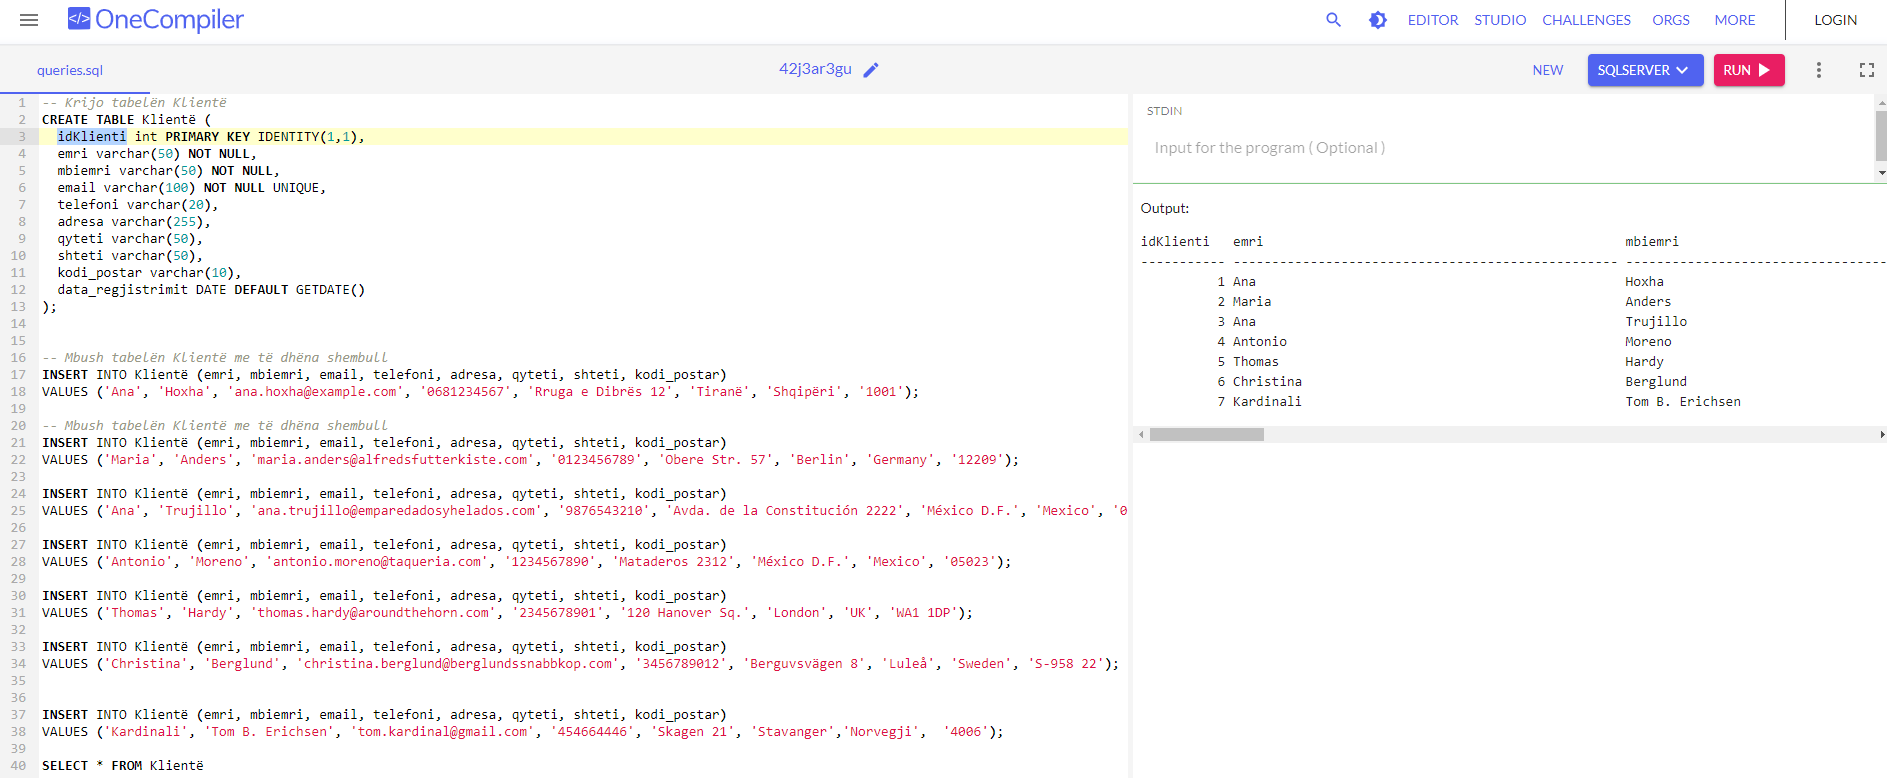
\includegraphics{./Figs/query30.png}
\end{frame}

\begin{frame}{Sintaksa INSERT INTO}
\phantomsection\label{sintaksa-insert-into-3}
\begin{itemize}
\item
  A e keni vënë re që nuk kemi futur ndonjë numër në fushën e ID-së së
  klientit?
\item
  Kolona \textbf{idKlienti} është një fushë me rritje automatike dhe do
  të gjenerohet automatikisht kur një rekord i ri futet në tabelë.
\end{itemize}
\end{frame}

\begin{frame}{Futja e të dhënave vetëm në kolonat e specifikuara}
\phantomsection\label{futja-e-tuxeb-dhuxebnave-vetuxebm-nuxeb-kolonat-e-specifikuara}
\begin{itemize}
\tightlist
\item
  Është gjithashtu e mundur që të futen të dhëna vetëm në kolona
  specifike.
\end{itemize}
\end{frame}

\begin{frame}{Futja e të dhënave vetëm në kolonat e specifikuara}
\phantomsection\label{futja-e-tuxeb-dhuxebnave-vetuxebm-nuxeb-kolonat-e-specifikuara-1}
\begin{itemize}
\tightlist
\item
  Deklarata e mëposhtme SQL do të fusë një rekord të ri, por fut vetëm
  të dhëna në kolonat ``emri'', ``qyteti'' dhe ``shteti''
\end{itemize}

(ID-ja e klientit do të përditësohet automatikisht):
\end{frame}

\begin{frame}[fragile]{Shembull}
\phantomsection\label{shembull-4}
\AddToHookNext{env/Highlighting/begin}{\tiny}

\begin{Shaded}
\begin{Highlighting}[]
\CommentTok{{-}{-} Mbush tabelën Klientë me të dhëna shtesë, duke siguruar që email{-}i të jetë unik ose i bosh}
\KeywordTok{INSERT} \KeywordTok{INTO}\NormalTok{ Klientë (emri, qyteti, shteti)}
\KeywordTok{VALUES}\NormalTok{ (}\StringTok{\textquotesingle{}John\textquotesingle{}}\NormalTok{, }\StringTok{\textquotesingle{}Wayne\textquotesingle{}}\NormalTok{, }\StringTok{\textquotesingle{}Albania\textquotesingle{}}\NormalTok{);}
\end{Highlighting}
\end{Shaded}
\end{frame}

\begin{frame}{Sintaksa INSERT INTO}
\phantomsection\label{sintaksa-insert-into-4}
\begin{itemize}
\tightlist
\item
  Zgjedhja nga tabela ``Klientë'' tani do të duket kështu:
\end{itemize}
\end{frame}

\begin{frame}{Shembull}
\phantomsection\label{shembull-5}
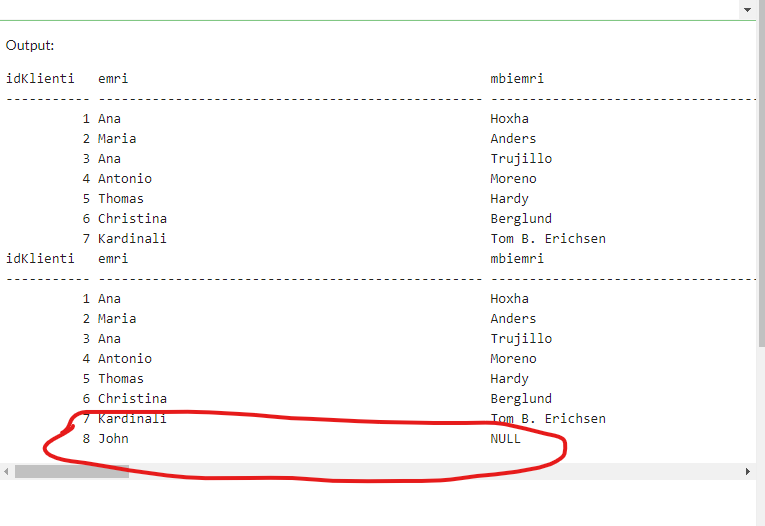
\includegraphics{./Figs/query31.png}
\end{frame}

\begin{frame}{Futja e shumë rreshtave}
\phantomsection\label{futja-e-shumuxeb-rreshtave}
\begin{itemize}
\item
  Është gjithashtu e mundur që të futen shumë rreshta në një deklaratë.
\item
  Për të futur shumë rreshta të dhënash, ne përdorim të njëjtën
  deklaratë \textbf{INSERT INTO}, por me vlera të shumta:
\end{itemize}
\end{frame}

\begin{frame}[fragile]{Shembull}
\phantomsection\label{shembull-6}
\AddToHookNext{env/Highlighting/begin}{\tiny}

\begin{Shaded}
\begin{Highlighting}[]
\KeywordTok{INSERT} \KeywordTok{INTO}\NormalTok{ Klientë (emri, mbiemri, adresa, qyteti, kodi\_postar, shteti, email)}
\KeywordTok{VALUES}
\NormalTok{(}\StringTok{\textquotesingle{}Cardinal\textquotesingle{}}\NormalTok{, }\StringTok{\textquotesingle{}Tom B. Erichsen\textquotesingle{}}\NormalTok{, }\StringTok{\textquotesingle{}Skagen 21\textquotesingle{}}\NormalTok{, }\StringTok{\textquotesingle{}Stavanger\textquotesingle{}}\NormalTok{, }\StringTok{\textquotesingle{}4006\textquotesingle{}}\NormalTok{, }\StringTok{\textquotesingle{}Norway\textquotesingle{}}\NormalTok{, }\StringTok{\textquotesingle{}cardinal.erichsen@norway.com\textquotesingle{}}\NormalTok{),}
\NormalTok{(}\StringTok{\textquotesingle{}Greasy Burger\textquotesingle{}}\NormalTok{, }\StringTok{\textquotesingle{}Per Olsen\textquotesingle{}}\NormalTok{, }\StringTok{\textquotesingle{}Gateveien 15\textquotesingle{}}\NormalTok{, }\StringTok{\textquotesingle{}Sandnes\textquotesingle{}}\NormalTok{, }\StringTok{\textquotesingle{}4306\textquotesingle{}}\NormalTok{, }\StringTok{\textquotesingle{}Norway\textquotesingle{}}\NormalTok{, }\StringTok{\textquotesingle{}greasy.burger@norway.com\textquotesingle{}}\NormalTok{),}
\NormalTok{(}\StringTok{\textquotesingle{}Tasty Tee\textquotesingle{}}\NormalTok{, }\StringTok{\textquotesingle{}Finn Egan\textquotesingle{}}\NormalTok{, }\StringTok{\textquotesingle{}Streetroad 19B\textquotesingle{}}\NormalTok{, }\StringTok{\textquotesingle{}Liverpool\textquotesingle{}}\NormalTok{, }\StringTok{\textquotesingle{}L1 0AA\textquotesingle{}}\NormalTok{, }\StringTok{\textquotesingle{}UK\textquotesingle{}}\NormalTok{, }\StringTok{\textquotesingle{}tasty.tee@uk.com\textquotesingle{}}\NormalTok{);}

\CommentTok{{-}{-} Kontrollo të dhënat e futura përsëri}
\KeywordTok{SELECT} \OperatorTok{*} \KeywordTok{FROM}\NormalTok{ Klientë;}
\end{Highlighting}
\end{Shaded}
\end{frame}

\begin{frame}{Sintaksa INSERT INTO}
\phantomsection\label{sintaksa-insert-into-5}
\begin{itemize}
\tightlist
\item
  Zgjedhja nga tabela ``Klientë'' tani do të duket kështu:
\end{itemize}
\end{frame}

\begin{frame}{Shembull}
\phantomsection\label{shembull-7}
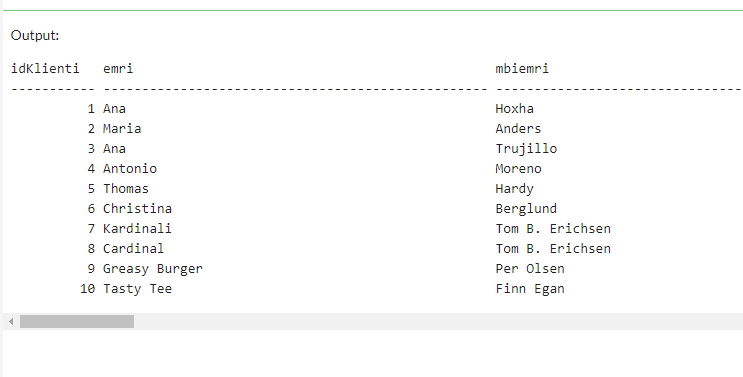
\includegraphics{./Figs/query32.png}
\end{frame}

\begin{frame}{Çfarë është një Vlerë NULL?}
\phantomsection\label{uxe7faruxeb-uxebshtuxeb-njuxeb-vleruxeb-null}
Një fushë me një vlerë NULL është një fushë pa vlerë.
\end{frame}

\begin{frame}{Çfarë është një Vlerë NULL?}
\phantomsection\label{uxe7faruxeb-uxebshtuxeb-njuxeb-vleruxeb-null-1}
\begin{itemize}
\item
  Nëse një fushë në një tabelë është opsionale, është e mundur të futni
  një rekord të ri ose të përditësoni një rekord pa shtuar një vlerë në
  këtë fushë.
\item
  Atëherë, fusha do të ruhet me një vlerë NULL.
\end{itemize}
\end{frame}

\begin{frame}{Çfarë është një Vlerë NULL?}
\phantomsection\label{uxe7faruxeb-uxebshtuxeb-njuxeb-vleruxeb-null-2}
\begin{itemize}
\item
  Një vlerë NULL është e ndryshme nga një vlerë zero ose një fushë që
  përmban hapësira.
\item
  Një fushë me një vlerë NULL është një fushë që është lënë bosh gjatë
  krijimit të rekordit!
\end{itemize}
\end{frame}

\begin{frame}{Si të Testoni për Vlera NULL?}
\phantomsection\label{si-tuxeb-testoni-puxebr-vlera-null}
\begin{itemize}
\item
  Nuk është e mundur të testoni për vlera NULL me operatorët e
  krahasimit, të tillë si =, \textless, ose \textless\textgreater.
\item
  Ne do të duhet të përdorim operatorët IS NULL dhe IS NOT NULL.
\end{itemize}
\end{frame}

\begin{frame}[fragile]{Sintaksa IS NULL}
\phantomsection\label{sintaksa-is-null}
\AddToHookNext{env/Highlighting/begin}{\tiny}

\begin{verbatim}
SELECT emrat_e_kolonave
FROM emri_i_tabelës
WHERE emri_i_kolonës IS NULL;
\end{verbatim}
\end{frame}

\begin{frame}[fragile]{Sintaksa IS NOT NULL}
\phantomsection\label{sintaksa-is-not-null}
\AddToHookNext{env/Highlighting/begin}{\tiny}

\begin{verbatim}
SELECT emrat_e_kolonave
FROM emri_i_tabelës
WHERE emri_i_kolonës IS NOT NULL;

\end{verbatim}
\end{frame}

\begin{frame}{Operator IS NULL}
\phantomsection\label{operator-is-null}
\begin{itemize}
\item
  Operatori IS NULL përdoret për të testuar për vlera bosh (vlera NULL).
\item
  SQL-ja e mëposhtme rendit të gjithë klientët me një vlerë NULL në
  fushën ``adresa'':
\end{itemize}
\end{frame}

\begin{frame}[fragile]{Tabela}
\phantomsection\label{tabela}
\AddToHookNext{env/Highlighting/begin}{\tiny}

\begin{Shaded}
\begin{Highlighting}[]
\CommentTok{{-}{-} Krijo tabelën Klientë}
\KeywordTok{CREATE} \KeywordTok{TABLE}\NormalTok{ Klientë (}
\NormalTok{  idKlienti }\DataTypeTok{int} \KeywordTok{PRIMARY} \KeywordTok{KEY}\NormalTok{ IDENTITY(}\DecValTok{1}\NormalTok{,}\DecValTok{1}\NormalTok{),}
\NormalTok{  emri }\DataTypeTok{varchar}\NormalTok{(}\DecValTok{50}\NormalTok{),}
\NormalTok{  mbiemri }\DataTypeTok{varchar}\NormalTok{(}\DecValTok{50}\NormalTok{),}
\NormalTok{  email }\DataTypeTok{varchar}\NormalTok{(}\DecValTok{100}\NormalTok{) }\KeywordTok{UNIQUE}\NormalTok{,}
\NormalTok{  telefoni }\DataTypeTok{varchar}\NormalTok{(}\DecValTok{20}\NormalTok{),}
\NormalTok{  adresa }\DataTypeTok{varchar}\NormalTok{(}\DecValTok{255}\NormalTok{),}
\NormalTok{  qyteti }\DataTypeTok{varchar}\NormalTok{(}\DecValTok{50}\NormalTok{),}
\NormalTok{  shteti }\DataTypeTok{varchar}\NormalTok{(}\DecValTok{50}\NormalTok{),}
\NormalTok{  kodi\_postar }\DataTypeTok{varchar}\NormalTok{(}\DecValTok{10}\NormalTok{),}
\NormalTok{  data\_regjistrimit }\DataTypeTok{DATE} \KeywordTok{DEFAULT}\NormalTok{ GETDATE()}
\NormalTok{);}
\end{Highlighting}
\end{Shaded}
\end{frame}

\begin{frame}[fragile]{Tabela}
\phantomsection\label{tabela-1}
\AddToHookNext{env/Highlighting/begin}{\tiny}

\begin{Shaded}
\begin{Highlighting}[]

\CommentTok{{-}{-} Mbush tabelën Klientë me të dhëna shembull, përfshirë disa me fusha adresa bosh}
\KeywordTok{INSERT} \KeywordTok{INTO}\NormalTok{ Klientë (emri, mbiemri, email, telefoni, adresa, qyteti, shteti, kodi\_postar)}
\KeywordTok{VALUES} 
\NormalTok{(}\StringTok{\textquotesingle{}Ana\textquotesingle{}}\NormalTok{, }\StringTok{\textquotesingle{}Hoxha\textquotesingle{}}\NormalTok{, }\StringTok{\textquotesingle{}ana.hoxha@example.com\textquotesingle{}}\NormalTok{, }\StringTok{\textquotesingle{}0681234567\textquotesingle{}}\NormalTok{, }\StringTok{\textquotesingle{}Rruga e Dibrës 12\textquotesingle{}}\NormalTok{, }\StringTok{\textquotesingle{}Tiranë\textquotesingle{}}\NormalTok{, }\StringTok{\textquotesingle{}Shqipëri\textquotesingle{}}\NormalTok{, }\StringTok{\textquotesingle{}1001\textquotesingle{}}\NormalTok{),}
\NormalTok{(}\StringTok{\textquotesingle{}Maria\textquotesingle{}}\NormalTok{, }\StringTok{\textquotesingle{}Anders\textquotesingle{}}\NormalTok{, }\StringTok{\textquotesingle{}maria.anders@alfredsfutterkiste.com\textquotesingle{}}\NormalTok{, }\StringTok{\textquotesingle{}0123456789\textquotesingle{}}\NormalTok{, }\KeywordTok{NULL}\NormalTok{, }\StringTok{\textquotesingle{}Berlin\textquotesingle{}}\NormalTok{, }\StringTok{\textquotesingle{}Gjermani\textquotesingle{}}\NormalTok{, }\StringTok{\textquotesingle{}12209\textquotesingle{}}\NormalTok{),}
\NormalTok{(}\StringTok{\textquotesingle{}Ana\textquotesingle{}}\NormalTok{, }\StringTok{\textquotesingle{}Trujillo\textquotesingle{}}\NormalTok{, }\StringTok{\textquotesingle{}ana.trujillo@emparedadosyhelados.com\textquotesingle{}}\NormalTok{, }\StringTok{\textquotesingle{}9876543210\textquotesingle{}}\NormalTok{, }\StringTok{\textquotesingle{}Avda. de la Constitución 2222\textquotesingle{}}\NormalTok{, }\StringTok{\textquotesingle{}México D.F.\textquotesingle{}}\NormalTok{, }\StringTok{\textquotesingle{}Meksikë\textquotesingle{}}\NormalTok{, }\StringTok{\textquotesingle{}05021\textquotesingle{}}\NormalTok{),}
\NormalTok{(}\StringTok{\textquotesingle{}Antonio\textquotesingle{}}\NormalTok{, }\StringTok{\textquotesingle{}Moreno\textquotesingle{}}\NormalTok{, }\StringTok{\textquotesingle{}antonio.moreno@taqueria.com\textquotesingle{}}\NormalTok{, }\StringTok{\textquotesingle{}1234567890\textquotesingle{}}\NormalTok{, }\StringTok{\textquotesingle{}Mataderos 2312\textquotesingle{}}\NormalTok{, }\StringTok{\textquotesingle{}México D.F.\textquotesingle{}}\NormalTok{, }\StringTok{\textquotesingle{}Meksikë\textquotesingle{}}\NormalTok{, }\StringTok{\textquotesingle{}05023\textquotesingle{}}\NormalTok{),}
\NormalTok{(}\StringTok{\textquotesingle{}Thomas\textquotesingle{}}\NormalTok{, }\StringTok{\textquotesingle{}Hardy\textquotesingle{}}\NormalTok{, }\StringTok{\textquotesingle{}thomas.hardy@aroundthehorn.com\textquotesingle{}}\NormalTok{, }\StringTok{\textquotesingle{}2345678901\textquotesingle{}}\NormalTok{, }\KeywordTok{NULL}\NormalTok{, }\StringTok{\textquotesingle{}London\textquotesingle{}}\NormalTok{, }\StringTok{\textquotesingle{}MB\textquotesingle{}}\NormalTok{, }\StringTok{\textquotesingle{}WA1 1DP\textquotesingle{}}\NormalTok{),}
\NormalTok{(}\StringTok{\textquotesingle{}Christina\textquotesingle{}}\NormalTok{, }\StringTok{\textquotesingle{}Berglund\textquotesingle{}}\NormalTok{, }\StringTok{\textquotesingle{}christina.berglund@berglundssnabbkop.com\textquotesingle{}}\NormalTok{, }\StringTok{\textquotesingle{}3456789012\textquotesingle{}}\NormalTok{, }\StringTok{\textquotesingle{}Berguvsvägen 8\textquotesingle{}}\NormalTok{, }\StringTok{\textquotesingle{}Luleå\textquotesingle{}}\NormalTok{, }\StringTok{\textquotesingle{}Suedi\textquotesingle{}}\NormalTok{, }\StringTok{\textquotesingle{}S{-}958 22\textquotesingle{}}\NormalTok{),}
\NormalTok{(}\StringTok{\textquotesingle{}Kardinali\textquotesingle{}}\NormalTok{, }\StringTok{\textquotesingle{}Tom B. Erichsen\textquotesingle{}}\NormalTok{, }\StringTok{\textquotesingle{}tom.kardinal@gmail.com\textquotesingle{}}\NormalTok{, }\StringTok{\textquotesingle{}454664446\textquotesingle{}}\NormalTok{, }\StringTok{\textquotesingle{}Skagen 21\textquotesingle{}}\NormalTok{, }\StringTok{\textquotesingle{}Stavanger\textquotesingle{}}\NormalTok{,}\StringTok{\textquotesingle{}Norvegji\textquotesingle{}}\NormalTok{, }\StringTok{\textquotesingle{}4006\textquotesingle{}}\NormalTok{),}
\NormalTok{(}\StringTok{\textquotesingle{}John\textquotesingle{}}\NormalTok{, }\StringTok{\textquotesingle{}Wayne\textquotesingle{}}\NormalTok{, }\KeywordTok{NULL}\NormalTok{, }\KeywordTok{NULL}\NormalTok{, }\KeywordTok{NULL}\NormalTok{, }\StringTok{\textquotesingle{}Wayne\textquotesingle{}}\NormalTok{, }\StringTok{\textquotesingle{}Albania\textquotesingle{}}\NormalTok{, }\KeywordTok{NULL}\NormalTok{);}
\end{Highlighting}
\end{Shaded}
\end{frame}

\begin{frame}[fragile]{Testimi për Vlera NULL}
\phantomsection\label{testimi-puxebr-vlera-null}
\AddToHookNext{env/Highlighting/begin}{\tiny}

\begin{Shaded}
\begin{Highlighting}[]
\KeywordTok{SELECT}\NormalTok{ emri, mbiemri, adresa}
\KeywordTok{FROM}\NormalTok{ Klientë}
\KeywordTok{WHERE}\NormalTok{ adresa }\KeywordTok{IS} \KeywordTok{NULL}\NormalTok{;}
\end{Highlighting}
\end{Shaded}
\end{frame}

\begin{frame}{Shembull}
\phantomsection\label{shembull-8}
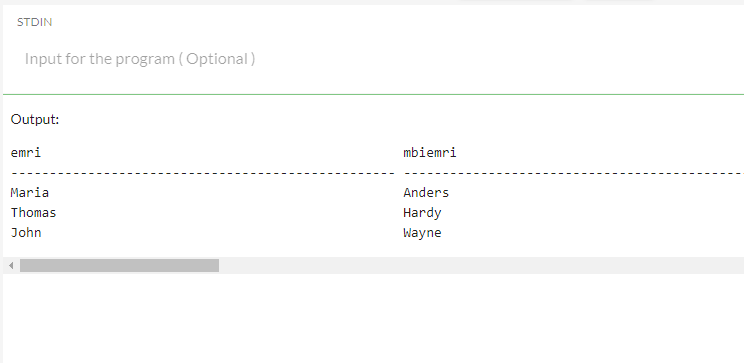
\includegraphics{./Figs/query33}
\end{frame}

\begin{frame}[fragile]{Testimi për Vlera NOT NULL}
\phantomsection\label{testimi-puxebr-vlera-not-null}
\AddToHookNext{env/Highlighting/begin}{\tiny}

\begin{Shaded}
\begin{Highlighting}[]
\KeywordTok{SELECT}\NormalTok{ emri, mbiemri, adresa}
\KeywordTok{FROM}\NormalTok{ Klientë}
\KeywordTok{WHERE}\NormalTok{ adresa }\KeywordTok{IS} \KeywordTok{NOT} \KeywordTok{NULL}\NormalTok{;}
\end{Highlighting}
\end{Shaded}
\end{frame}

\begin{frame}{Shembull}
\phantomsection\label{shembull-9}
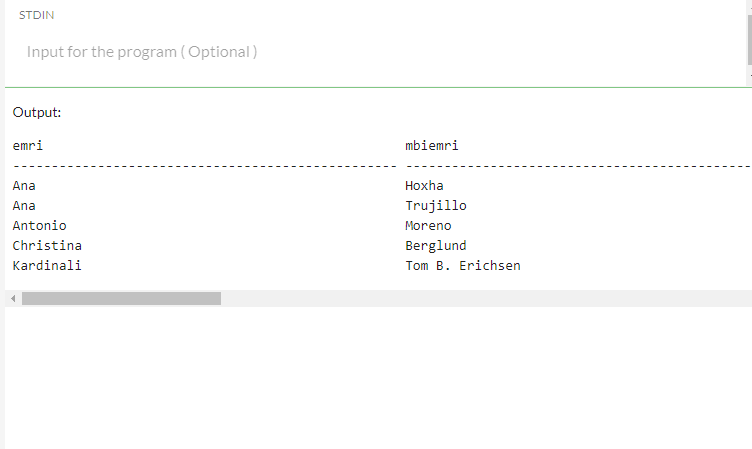
\includegraphics{./Figs/query34}
\end{frame}

\begin{frame}[fragile]{Deklarata SQL UPDATE}
\phantomsection\label{deklarata-sql-update}
Deklarata \texttt{UPDATE} përdoret për të modifikuar rekordet ekzistuese
në një tabelë.
\end{frame}

\begin{frame}[fragile]{Sintaksa UPDATE}
\phantomsection\label{sintaksa-update}
\begin{Shaded}
\begin{Highlighting}[]
\KeywordTok{UPDATE}\NormalTok{ emri\_i\_tabelës}
\KeywordTok{SET}\NormalTok{ kolona1 }\OperatorTok{=}\NormalTok{ vlera1, kolona2 }\OperatorTok{=}\NormalTok{ vlera2, }\OperatorTok{..}\NormalTok{.}
\KeywordTok{WHERE}\NormalTok{ kushti;}
\end{Highlighting}
\end{Shaded}
\end{frame}

\begin{frame}{Sintaksa UPDATE}
\phantomsection\label{sintaksa-update-1}
\begin{itemize}
\item
  Bëni kujdes kur përditësoni rekordet në një tabelë!
\item
  Vini re klauzolën WHERE në deklaratën UPDATE. Klauzola WHERE
  specifikon cilat rekorde do të përditësohen.
\item
  Nëse e lini jashtë klauzolën WHERE, të gjitha rekordet në tabelë do të
  përditësohen!
\end{itemize}
\end{frame}

\begin{frame}[fragile]{Përditësimi i Një Rekordi}
\phantomsection\label{puxebrdituxebsimi-i-njuxeb-rekordi}
Deklarata SQL më poshtë përditëson klientin e parë (idKlienti = 1) me
një kontakt të ri dhe një qytet të ri.

\AddToHookNext{env/Highlighting/begin}{\tiny}

\begin{Shaded}
\begin{Highlighting}[]
\KeywordTok{UPDATE}\NormalTok{ Klientë}
\KeywordTok{SET}\NormalTok{ mbiemri }\OperatorTok{=} \StringTok{\textquotesingle{}Schmidt\textquotesingle{}}\NormalTok{, qyteti }\OperatorTok{=} \StringTok{\textquotesingle{}Frankfurt\textquotesingle{}}
\KeywordTok{WHERE}\NormalTok{ idKlienti }\OperatorTok{=} \DecValTok{1}\NormalTok{;}
\end{Highlighting}
\end{Shaded}
\end{frame}

\begin{frame}{Sintaksa INSERT INTO}
\phantomsection\label{sintaksa-insert-into-6}
\begin{itemize}
\tightlist
\item
  Zgjedhja nga tabela ``Klientë'' tani do të duket kështu:
\end{itemize}
\end{frame}

\begin{frame}{Shembull}
\phantomsection\label{shembull-10}
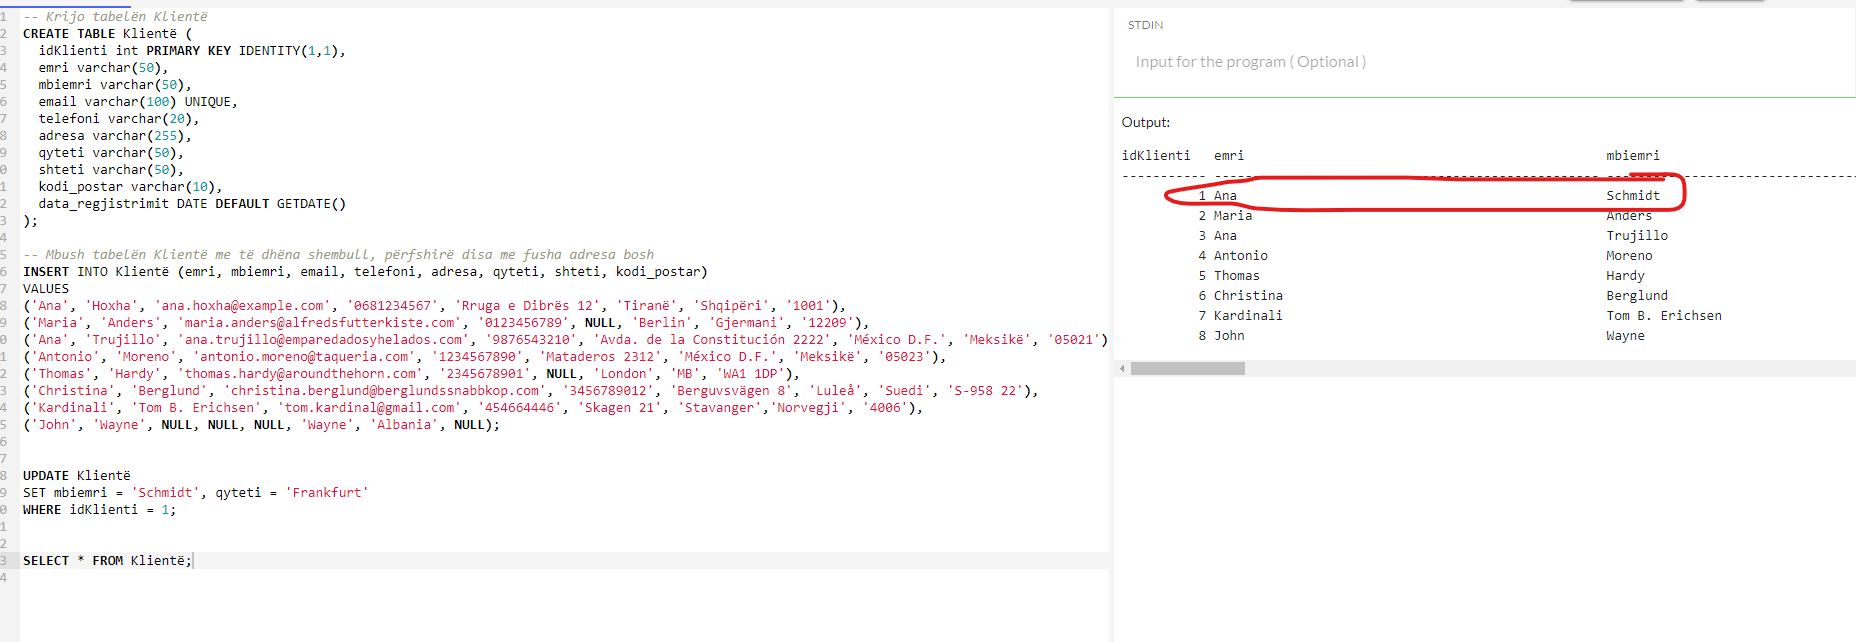
\includegraphics{./Figs/query35.png}
\end{frame}

\begin{frame}{Përditësimi i Rekordeve të Shumta}
\phantomsection\label{puxebrdituxebsimi-i-rekordeve-tuxeb-shumta}
\begin{itemize}
\item
  Është klauzola \textbf{WHERE} që përcakton se sa rekorde do të
  përditësohen.
\item
  Deklarata SQL më poshtë do të përditësojë mbiemrin në ``Juan'' për të
  gjitha rekordet ku shteti është ``Meksikë'':
\end{itemize}
\end{frame}

\begin{frame}[fragile]{Përditësimi i Rekordeve të Shumta}
\phantomsection\label{puxebrdituxebsimi-i-rekordeve-tuxeb-shumta-1}
\AddToHookNext{env/Highlighting/begin}{\tiny}

\begin{Shaded}
\begin{Highlighting}[]
\KeywordTok{UPDATE}\NormalTok{ Klientë}
\KeywordTok{SET}\NormalTok{ mbiemri }\OperatorTok{=} \StringTok{\textquotesingle{}Juan\textquotesingle{}}
\KeywordTok{WHERE}\NormalTok{ shteti }\OperatorTok{=} \StringTok{\textquotesingle{}Meksikë\textquotesingle{}}\NormalTok{;}
\end{Highlighting}
\end{Shaded}
\end{frame}

\begin{frame}{Sintaksa INSERT INTO}
\phantomsection\label{sintaksa-insert-into-7}
\begin{itemize}
\tightlist
\item
  Zgjedhja nga tabela ``Klientë'' tani do të duket kështu:
\end{itemize}
\end{frame}

\begin{frame}{Shembull}
\phantomsection\label{shembull-11}
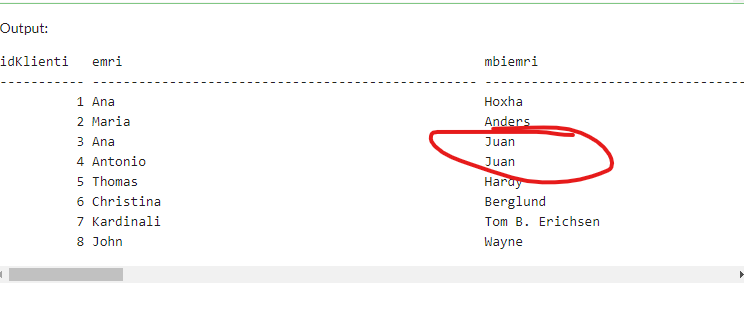
\includegraphics{./Figs/query36.png}
\end{frame}

\begin{frame}{Paralajmërim për Përditësimin}
\phantomsection\label{paralajmuxebrim-puxebr-puxebrdituxebsimin}
\begin{itemize}
\item
  Bëni kujdes kur përditësoni rekordet.
\item
  Nëse e lini jashtë klauzolën WHERE, të gjitha rekordet do të
  përditësohen!
\end{itemize}
\end{frame}

\begin{frame}[fragile]{Pa Klauzolën WHERE}
\phantomsection\label{pa-klauzoluxebn-where}
\AddToHookNext{env/Highlighting/begin}{\tiny}

\begin{Shaded}
\begin{Highlighting}[]
\KeywordTok{UPDATE}\NormalTok{ Klientë}
\KeywordTok{SET}\NormalTok{ mbiemri }\OperatorTok{=} \StringTok{\textquotesingle{}Juan\textquotesingle{}}\NormalTok{;}
\end{Highlighting}
\end{Shaded}
\end{frame}

\begin{frame}{Pa Klauzolën WHERE}
\phantomsection\label{pa-klauzoluxebn-where-1}
\begin{itemize}
\tightlist
\item
  Zgjedhja nga tabela ``Klientë'' tani do të duket kështu:
\end{itemize}
\end{frame}

\begin{frame}{Shembull}
\phantomsection\label{shembull-12}
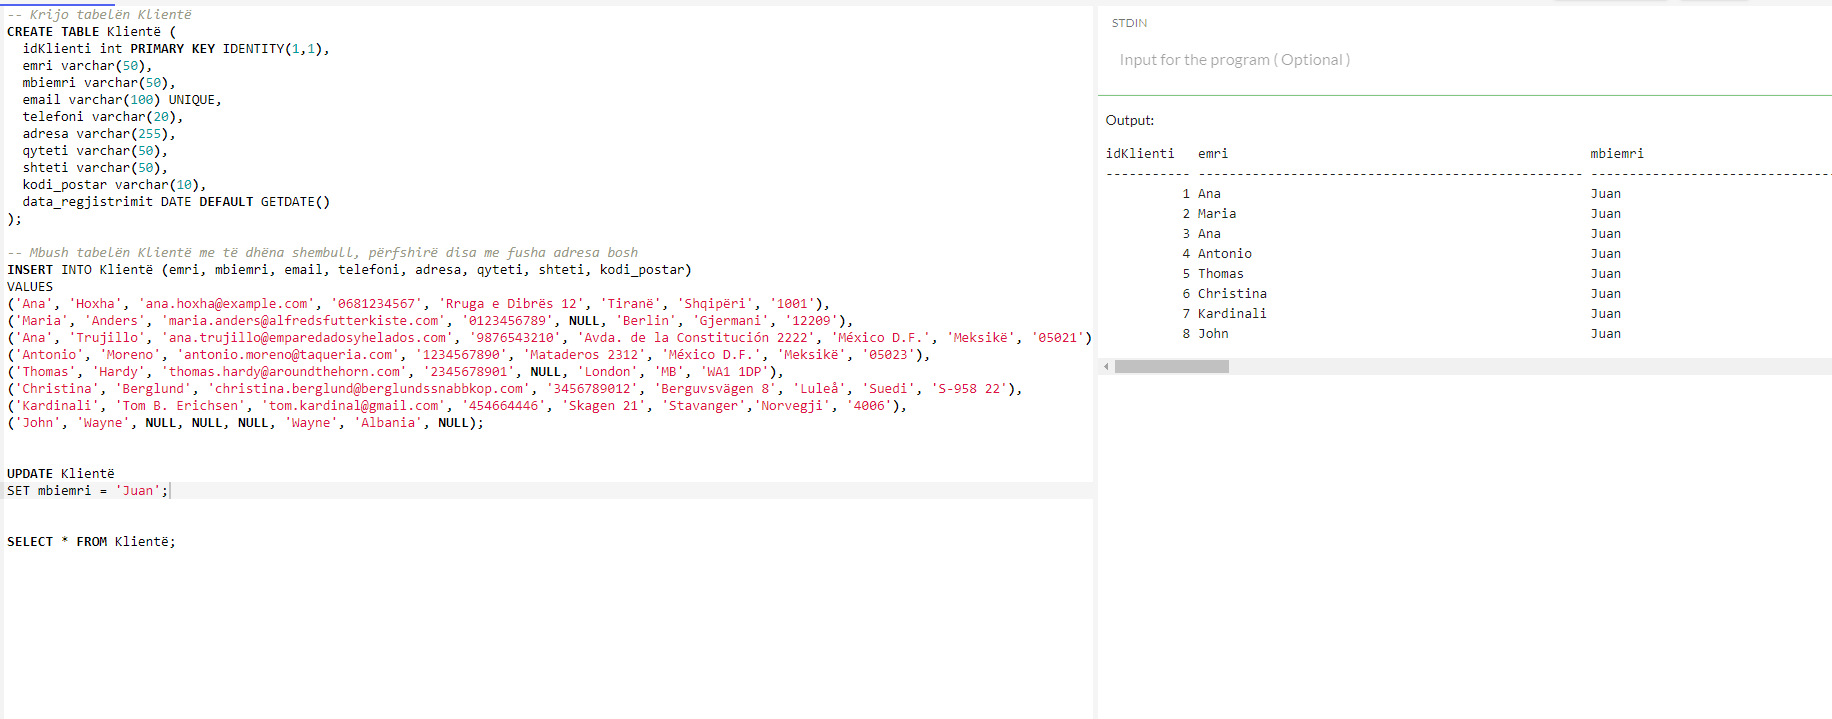
\includegraphics{./Figs/query37.png}
\end{frame}

\begin{frame}[fragile]{Deklarata SQL DELETE}
\phantomsection\label{deklarata-sql-delete}
Deklarata \texttt{DELETE} përdoret për të fshirë rekordet ekzistuese në
një tabelë.
\end{frame}

\begin{frame}[fragile]{Sintaksa DELETE}
\phantomsection\label{sintaksa-delete}
\begin{Shaded}
\begin{Highlighting}[]
\KeywordTok{DELETE} \KeywordTok{FROM}\NormalTok{ emri\_i\_tabelës }\KeywordTok{WHERE}\NormalTok{ kushti;}
\end{Highlighting}
\end{Shaded}
\end{frame}

\begin{frame}{Sintaksa DELETE}
\phantomsection\label{sintaksa-delete-1}
\begin{itemize}
\item
  Bëni kujdes kur fshini rekorde në një tabelë!
\item
  Vini re klauzolën WHERE në deklaratën DELETE.
\item
  Klauzola WHERE specifikon cilat rekorde do të fshihen.
\item
  Nëse e lini jashtë klauzolën WHERE, të gjitha rekordet në tabelë do të
  fshihen!
\end{itemize}
\end{frame}

\begin{frame}{Shembulli DELETE}
\phantomsection\label{shembulli-delete}
\begin{itemize}
\tightlist
\item
  Deklarata SQL më poshtë fshin klientin ``Alfreds Futterkiste'' nga
  tabela Klientë:
\end{itemize}
\end{frame}

\begin{frame}[fragile]{Shembulli DELETE}
\phantomsection\label{shembulli-delete-1}
\AddToHookNext{env/Highlighting/begin}{\tiny}

\begin{Shaded}
\begin{Highlighting}[]
\KeywordTok{DELETE} \KeywordTok{FROM}\NormalTok{ Klientë }\KeywordTok{WHERE}\NormalTok{ emri}\OperatorTok{=}\StringTok{\textquotesingle{}John\textquotesingle{}} \KeywordTok{AND}\NormalTok{ mbiemri}\OperatorTok{=}\StringTok{\textquotesingle{}Wayne\textquotesingle{}}\NormalTok{;}
\end{Highlighting}
\end{Shaded}
\end{frame}

\begin{frame}{Shembulli DELETE}
\phantomsection\label{shembulli-delete-2}
\begin{itemize}
\tightlist
\item
  Zgjedhja nga tabela ``Klientë'' tani do të duket kështu:
\end{itemize}
\end{frame}

\begin{frame}{Shembulli DELETE}
\phantomsection\label{shembulli-delete-3}
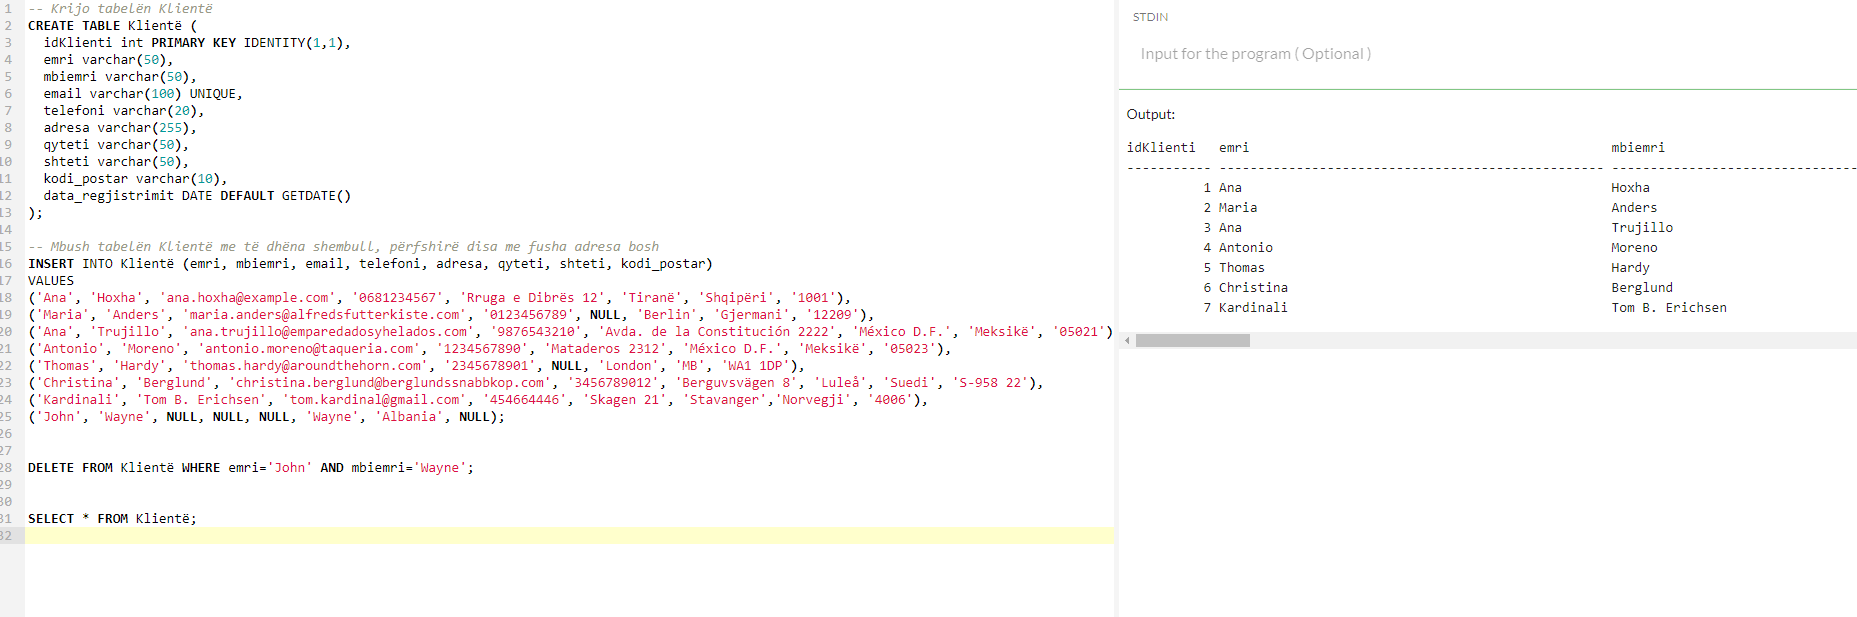
\includegraphics{./Figs/query38.png}
\end{frame}

\begin{frame}{Fshirja e të Gjitha Rekordeve}
\phantomsection\label{fshirja-e-tuxeb-gjitha-rekordeve}
\begin{itemize}
\item
  Është e mundur të fshini të gjitha rreshtat në një tabelë pa e fshirë
  tabelën.
\item
  Kjo do të thotë që struktura e tabelës, atributet dhe indekset do të
  mbeten të paprekura:
\end{itemize}
\end{frame}

\begin{frame}[fragile]{Fshirja e të Gjitha Rekordeve}
\phantomsection\label{fshirja-e-tuxeb-gjitha-rekordeve-1}
\begin{Shaded}
\begin{Highlighting}[]
\KeywordTok{DELETE} \KeywordTok{FROM}\NormalTok{ emri\_i\_tabelës;}
\end{Highlighting}
\end{Shaded}
\end{frame}

\begin{frame}{Fshirja e të Gjitha Rekordeve}
\phantomsection\label{fshirja-e-tuxeb-gjitha-rekordeve-2}
\begin{itemize}
\tightlist
\item
  Deklarata SQL më poshtë fshin të gjitha rreshtat në tabelën Klientë,
  pa e fshirë tabelën:
\end{itemize}
\end{frame}

\begin{frame}[fragile]{Fshirja e të Gjitha Rekordeve}
\phantomsection\label{fshirja-e-tuxeb-gjitha-rekordeve-3}
\AddToHookNext{env/Highlighting/begin}{\tiny}

\begin{Shaded}
\begin{Highlighting}[]
\KeywordTok{DELETE} \KeywordTok{FROM}\NormalTok{ Klientë;}
\end{Highlighting}
\end{Shaded}
\end{frame}

\begin{frame}{Fshirja e të Gjitha Rekordeve}
\phantomsection\label{fshirja-e-tuxeb-gjitha-rekordeve-4}
\begin{itemize}
\tightlist
\item
  Zgjedhja nga tabela ``Klientë'' tani do të duket kështu:
\end{itemize}
\end{frame}

\begin{frame}{Fshirja e të Gjitha Rekordeve}
\phantomsection\label{fshirja-e-tuxeb-gjitha-rekordeve-5}
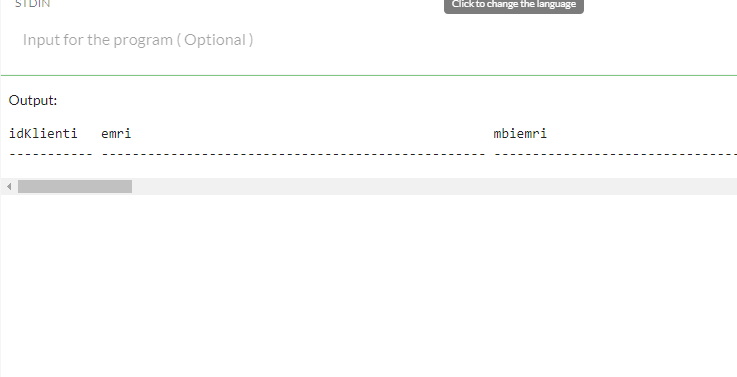
\includegraphics{./Figs/query39.png}
\end{frame}

\begin{frame}[fragile]{Fshirja e një Tabele}
\phantomsection\label{fshirja-e-njuxeb-tabele}
Për të fshirë plotësisht një tabelë, përdorni deklaratën DROP TABLE:

\AddToHookNext{env/Highlighting/begin}{\tiny}

\begin{Shaded}
\begin{Highlighting}[]
\KeywordTok{DROP} \KeywordTok{TABLE}\NormalTok{ Klientë;}
\end{Highlighting}
\end{Shaded}
\end{frame}

\begin{frame}[fragile]{Klauzola SQL SELECT TOP}
\phantomsection\label{klauzola-sql-select-top}
\begin{itemize}
\item
  Klauzola \texttt{SELECT\ TOP} përdoret për të specifikuar numrin e
  rekordeve që do të kthehen.
\item
  Klauzola \texttt{SELECT\ TOP} është e dobishme në tabelat e mëdha me
  mijëra rekorde.
\item
  Kthimi i një numri të madh rekordesh mund të ndikojë në performancë.
\end{itemize}
\end{frame}

\begin{frame}[fragile]{Sintaksa për SQL Server}
\phantomsection\label{sintaksa-puxebr-sql-server}
\AddToHookNext{env/Highlighting/begin}{\tiny}

\begin{Shaded}
\begin{Highlighting}[]
\KeywordTok{SELECT}\NormalTok{ TOP numri|përqindja kolona(t)}
\KeywordTok{FROM}\NormalTok{ emri\_i\_tabelës}
\KeywordTok{WHERE}\NormalTok{ kushti;}
\end{Highlighting}
\end{Shaded}
\end{frame}

\begin{frame}{Shembull}
\phantomsection\label{shembull-13}
\begin{itemize}
\tightlist
\item
  Zgjedh vetëm tre rekordet e para të tabelës Klientë:
\end{itemize}
\end{frame}

\begin{frame}[fragile]{Shembull}
\phantomsection\label{shembull-14}
\AddToHookNext{env/Highlighting/begin}{\tiny}

\begin{Shaded}
\begin{Highlighting}[]
\KeywordTok{SELECT}\NormalTok{ TOP }\DecValTok{3} \OperatorTok{*} \KeywordTok{FROM}\NormalTok{ Klientë;}
\end{Highlighting}
\end{Shaded}
\end{frame}

\begin{frame}{Shembull}
\phantomsection\label{shembull-15}
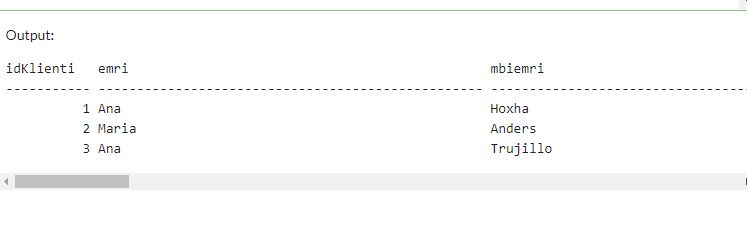
\includegraphics{./Figs/query40.png}
\end{frame}

\begin{frame}[fragile]{Shembulli i Përqindjes në SQL Server}
\phantomsection\label{shembulli-i-puxebrqindjes-nuxeb-sql-server}
\begin{itemize}
\tightlist
\item
  Zgjedh 50\% të parë të rekordeve nga tabela Klientë:
\end{itemize}

\AddToHookNext{env/Highlighting/begin}{\tiny}

\begin{Shaded}
\begin{Highlighting}[]
\KeywordTok{SELECT}\NormalTok{ TOP }\DecValTok{50} \KeywordTok{PERCENT} \OperatorTok{*} \KeywordTok{FROM}\NormalTok{ Klientë;}
\end{Highlighting}
\end{Shaded}
\end{frame}

\begin{frame}{Shtimi i Klauzolës WHERE}
\phantomsection\label{shtimi-i-klauzoluxebs-where}
\begin{itemize}
\tightlist
\item
  Zgjedh tre rekordet e para nga tabela Klientë, ku shteti është
  ``Gjermani'':
\end{itemize}
\end{frame}

\begin{frame}[fragile]{Shtimi i Klauzolës WHERE}
\phantomsection\label{shtimi-i-klauzoluxebs-where-1}
\AddToHookNext{env/Highlighting/begin}{\tiny}

\begin{Shaded}
\begin{Highlighting}[]
\KeywordTok{SELECT}\NormalTok{ TOP }\DecValTok{3} \OperatorTok{*} \KeywordTok{FROM}\NormalTok{ Klientë}
\KeywordTok{WHERE}\NormalTok{ shteti}\OperatorTok{=}\StringTok{\textquotesingle{}Gjermani\textquotesingle{}}\NormalTok{;}
\end{Highlighting}
\end{Shaded}
\end{frame}

\begin{frame}{Shembull}
\phantomsection\label{shembull-16}
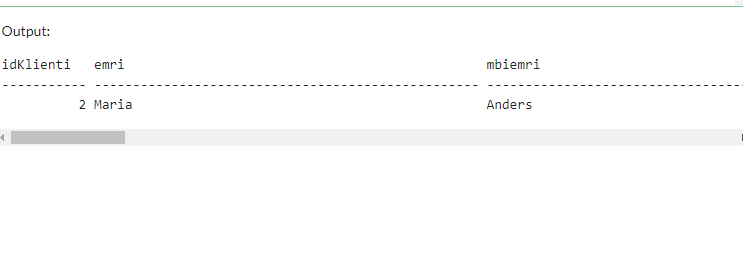
\includegraphics{./Figs/query41.png}
\end{frame}

\begin{frame}{Shtimi i Fjalës Kyçe ORDER BY}
\phantomsection\label{shtimi-i-fjaluxebs-kyuxe7e-order-by}
\begin{itemize}
\tightlist
\item
  Shtoni fjalën kyçe \textbf{ORDER BY} kur dëshironi të renditni
  rezultatin dhe të ktheni tre rekordet e para të rezultatit të
  renditur.
\end{itemize}
\end{frame}

\begin{frame}[fragile]{Shembull}
\phantomsection\label{shembull-17}
\begin{itemize}
\tightlist
\item
  Renditni rezultatin në mënyrë alfabetike të kundërt sipas emrit, dhe
  ktheni tre rekordet e para:
\end{itemize}

\AddToHookNext{env/Highlighting/begin}{\tiny}

\begin{Shaded}
\begin{Highlighting}[]
\KeywordTok{SELECT}\NormalTok{ TOP }\DecValTok{3} \OperatorTok{*} \KeywordTok{FROM}\NormalTok{ Klientë}
\KeywordTok{ORDER} \KeywordTok{BY}\NormalTok{ emri }\KeywordTok{DESC}\NormalTok{;}
\end{Highlighting}
\end{Shaded}
\end{frame}

\begin{frame}{Shembull}
\phantomsection\label{shembull-18}
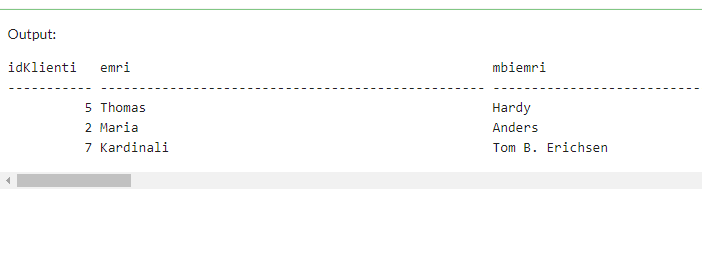
\includegraphics{./Figs/query42.png}
\end{frame}

\begin{frame}{Funksionet Agreguese në SQL}
\phantomsection\label{funksionet-agreguese-nuxeb-sql}
\begin{itemize}
\tightlist
\item
  Një funksion agregues është një funksion që kryen një llogaritje mbi
  një grup vlerash dhe kthen një vlerë të vetme.
\end{itemize}
\end{frame}

\begin{frame}[fragile]{Funksionet Agreguese në SQL}
\phantomsection\label{funksionet-agreguese-nuxeb-sql-1}
\begin{itemize}
\item
  Funksionet agreguese shpesh përdoren me klauzolën \texttt{GROUP\ BY}
  të deklaratës \texttt{SELECT}.
\item
  Klauzola \texttt{GROUP\ BY} ndan grupin e rezultateve në grupe vlerash
  dhe funksioni agregues mund të përdoret për të kthyer një vlerë të
  vetme për secilin grup.
\end{itemize}
\end{frame}

\begin{frame}{Funksionet Agreguese në SQL}
\phantomsection\label{funksionet-agreguese-nuxeb-sql-2}
Funksionet agreguese më të përdorura në SQL janë:

\begin{itemize}
\tightlist
\item
  \textbf{MIN()} - kthen vlerën më të vogël brenda kolonës së zgjedhur
\item
  \textbf{MAX()} - kthen vlerën më të madhe brenda kolonës së zgjedhur
\item
  \textbf{COUNT()} - kthen numrin e rreshtave në një grup
\item
  \textbf{SUM()} - kthen shumën totale të një kolone numerike
\item
  \textbf{AVG()} - kthen vlerën mesatare të një kolone numerike
\end{itemize}
\end{frame}

\begin{frame}{Funksionet Agreguese në SQL}
\phantomsection\label{funksionet-agreguese-nuxeb-sql-3}
Funksionet agreguese injorojnë vlerat null (përveç \textbf{COUNT()}).
\end{frame}

\begin{frame}[fragile]{Funksionet SQL MIN() dhe MAX()}
\phantomsection\label{funksionet-sql-min-dhe-max}
\begin{itemize}
\item
  Funksioni \texttt{MIN()} kthen vlerën më të vogël të kolonës së
  zgjedhur.
\item
  Funksioni \texttt{MAX()} kthen vlerën më të madhe të kolonës së
  zgjedhur.
\end{itemize}
\end{frame}

\begin{frame}[fragile]{Shembull për MIN()}
\phantomsection\label{shembull-puxebr-min}
Gjeni çmimin më të ulët në kolonën \texttt{Çmimi}:

\AddToHookNext{env/Highlighting/begin}{\tiny}

\begin{Shaded}
\begin{Highlighting}[]
\KeywordTok{SELECT} \FunctionTok{MIN}\NormalTok{(Çmimi)}
\KeywordTok{FROM}\NormalTok{ Produkte;}
\end{Highlighting}
\end{Shaded}
\end{frame}

\begin{frame}[fragile]{Tabela}
\phantomsection\label{tabela-2}
\AddToHookNext{env/Highlighting/begin}{\tiny}

\begin{Shaded}
\begin{Highlighting}[]
\CommentTok{{-}{-} Krijo tabelën Produkte}
\KeywordTok{CREATE} \KeywordTok{TABLE}\NormalTok{ Produkte (}
\NormalTok{  ProduktID }\DataTypeTok{int} \KeywordTok{PRIMARY} \KeywordTok{KEY}\NormalTok{ IDENTITY(}\DecValTok{1}\NormalTok{,}\DecValTok{1}\NormalTok{),}
\NormalTok{  EmriProduktit }\DataTypeTok{varchar}\NormalTok{(}\DecValTok{255}\NormalTok{) }\KeywordTok{NOT} \KeywordTok{NULL}\NormalTok{,}
\NormalTok{  FurnizuesiID }\DataTypeTok{int} \KeywordTok{NOT} \KeywordTok{NULL}\NormalTok{,}
\NormalTok{  KategoriaID }\DataTypeTok{int} \KeywordTok{NOT} \KeywordTok{NULL}\NormalTok{,}
\NormalTok{  Njesia }\DataTypeTok{varchar}\NormalTok{(}\DecValTok{255}\NormalTok{) }\KeywordTok{NOT} \KeywordTok{NULL}\NormalTok{,}
\NormalTok{  Çmimi }\DataTypeTok{decimal}\NormalTok{(}\DecValTok{10}\NormalTok{, }\DecValTok{2}\NormalTok{) }\KeywordTok{NOT} \KeywordTok{NULL}
\NormalTok{);}
\end{Highlighting}
\end{Shaded}
\end{frame}

\begin{frame}[fragile]{Tabela}
\phantomsection\label{tabela-3}
\AddToHookNext{env/Highlighting/begin}{\tiny}

\begin{Shaded}
\begin{Highlighting}[]
\CommentTok{{-}{-} Mbush tabelën Produkte me të dhëna shembull}
\KeywordTok{INSERT} \KeywordTok{INTO}\NormalTok{ Produkte (EmriProduktit, FurnizuesiID, KategoriaID, Njesia, Çmimi)}
\KeywordTok{VALUES} 
\NormalTok{(}\StringTok{\textquotesingle{}Chais\textquotesingle{}}\NormalTok{, }\DecValTok{1}\NormalTok{, }\DecValTok{1}\NormalTok{, }\StringTok{\textquotesingle{}10 kuti x 20 qese\textquotesingle{}}\NormalTok{, }\FloatTok{18.00}\NormalTok{),}
\NormalTok{(}\StringTok{\textquotesingle{}Chang\textquotesingle{}}\NormalTok{, }\DecValTok{1}\NormalTok{, }\DecValTok{1}\NormalTok{, }\StringTok{\textquotesingle{}24 {-} 12 oz shishe\textquotesingle{}}\NormalTok{, }\FloatTok{19.00}\NormalTok{),}
\NormalTok{(}\StringTok{\textquotesingle{}Aniseed Syrup\textquotesingle{}}\NormalTok{, }\DecValTok{1}\NormalTok{, }\DecValTok{2}\NormalTok{, }\StringTok{\textquotesingle{}12 {-} 550 ml shishe\textquotesingle{}}\NormalTok{, }\FloatTok{10.00}\NormalTok{),}
\NormalTok{(}\StringTok{\textquotesingle{}Chef Anton}\CharTok{\textquotesingle{}\textquotesingle{}}\StringTok{s Cajun Seasoning\textquotesingle{}}\NormalTok{, }\DecValTok{2}\NormalTok{, }\DecValTok{2}\NormalTok{, }\StringTok{\textquotesingle{}48 {-} 6 oz kavanoza\textquotesingle{}}\NormalTok{, }\FloatTok{22.00}\NormalTok{),}
\NormalTok{(}\StringTok{\textquotesingle{}Chef Anton}\CharTok{\textquotesingle{}\textquotesingle{}}\StringTok{s Gumbo Mix\textquotesingle{}}\NormalTok{, }\DecValTok{2}\NormalTok{, }\DecValTok{2}\NormalTok{, }\StringTok{\textquotesingle{}36 kuti\textquotesingle{}}\NormalTok{, }\FloatTok{21.35}\NormalTok{);}
\end{Highlighting}
\end{Shaded}
\end{frame}

\begin{frame}[fragile]{Shembull për MAX()}
\phantomsection\label{shembull-puxebr-max}
Gjeni çmimin më të lartë në kolonën Çmimi:

\begin{Shaded}
\begin{Highlighting}[]
\KeywordTok{SELECT} \FunctionTok{MAX}\NormalTok{(Çmimi)}
\KeywordTok{FROM}\NormalTok{ Produkte;}
\end{Highlighting}
\end{Shaded}
\end{frame}

\begin{frame}{Shembull}
\phantomsection\label{shembull-19}
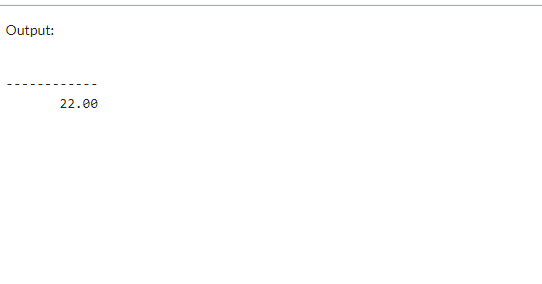
\includegraphics{./Figs/query43.png}
\end{frame}

\begin{frame}{Përcaktoni Emrin e Kolonës (Alias)}
\phantomsection\label{puxebrcaktoni-emrin-e-kolonuxebs-alias}
\begin{itemize}
\item
  Kur përdorni MIN() ose MAX(), kolona e kthyer nuk do të ketë një emër
  përshkrues.
\item
  Për t'i dhënë kolonës një emër përshkrues, përdorni fjalën kyçe AS:
\end{itemize}
\end{frame}

\begin{frame}[fragile]{Përcaktoni Emrin e Kolonës (Alias)}
\phantomsection\label{puxebrcaktoni-emrin-e-kolonuxebs-alias-1}
\AddToHookNext{env/Highlighting/begin}{\tiny}

\begin{Shaded}
\begin{Highlighting}[]
\KeywordTok{SELECT} \FunctionTok{MIN}\NormalTok{(Çmimi) }\KeywordTok{AS}\NormalTok{ ÇmimiMeIUlët}
\KeywordTok{FROM}\NormalTok{ Produkte;}
\end{Highlighting}
\end{Shaded}
\end{frame}

\begin{frame}{Shembull}
\phantomsection\label{shembull-20}
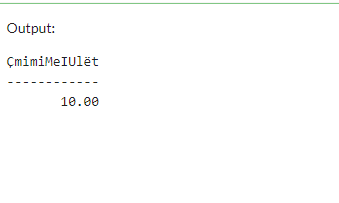
\includegraphics{./Figs/query44.png}
\end{frame}

\begin{frame}{Përdorni MIN() me GROUP BY}
\phantomsection\label{puxebrdorni-min-me-group-by}
Këtu përdorim funksionin MIN() dhe klauzolën GROUP BY, për të kthyer
çmimin më të ulët për secilën kategori në tabelën Produkte:
\end{frame}

\begin{frame}[fragile]{Përdorni MIN() me GROUP BY}
\phantomsection\label{puxebrdorni-min-me-group-by-1}
\AddToHookNext{env/Highlighting/begin}{\tiny}

\begin{Shaded}
\begin{Highlighting}[]
\KeywordTok{SELECT} \FunctionTok{MIN}\NormalTok{(Çmimi) }\KeywordTok{AS}\NormalTok{ ÇmimiMeIUlët, KategoriaID}
\KeywordTok{FROM}\NormalTok{ Produkte}
\KeywordTok{GROUP} \KeywordTok{BY}\NormalTok{ KategoriaID;}
\end{Highlighting}
\end{Shaded}
\end{frame}

\begin{frame}{Shembull}
\phantomsection\label{shembull-21}
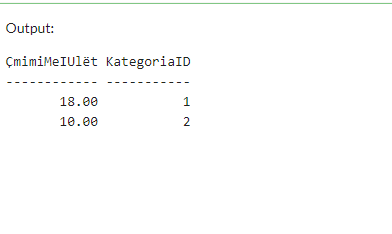
\includegraphics{./Figs/query45.png}
\end{frame}

\begin{frame}[fragile]{Funksioni SQL COUNT()}
\phantomsection\label{funksioni-sql-count}
\begin{itemize}
\tightlist
\item
  Funksioni \texttt{COUNT()} kthen numrin e rreshtave që përputhen me
  një kriter të specifikuar.
\end{itemize}
\end{frame}

\begin{frame}[fragile]{Shembull}
\phantomsection\label{shembull-22}
Gjeni numrin total të rreshtave në tabelën \texttt{Produkte}:

\AddToHookNext{env/Highlighting/begin}{\tiny}

\begin{Shaded}
\begin{Highlighting}[]
\KeywordTok{SELECT} \FunctionTok{COUNT}\NormalTok{(}\OperatorTok{*}\NormalTok{)}
\KeywordTok{FROM}\NormalTok{ Produkte;}
\end{Highlighting}
\end{Shaded}
\end{frame}

\begin{frame}{Shembull}
\phantomsection\label{shembull-23}
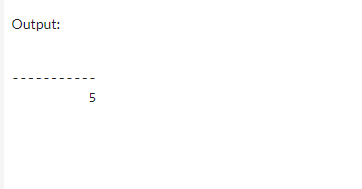
\includegraphics{./Figs/query46.png}
\end{frame}

\begin{frame}[fragile]{Sintaksa}
\phantomsection\label{sintaksa}
\AddToHookNext{env/Highlighting/begin}{\tiny}

\begin{Shaded}
\begin{Highlighting}[]
\KeywordTok{SELECT} \FunctionTok{COUNT}\NormalTok{(emri\_i\_kolonës)}
\KeywordTok{FROM}\NormalTok{ emri\_i\_tabelës}
\KeywordTok{WHERE}\NormalTok{ kushti;}
\end{Highlighting}
\end{Shaded}
\end{frame}

\begin{frame}{Përcaktoni Emrin e Kolonës}
\phantomsection\label{puxebrcaktoni-emrin-e-kolonuxebs}
\begin{itemize}
\item
  Ju mund të përcaktoni një emër kolone në vend të simbolit yll ().
\item
  Nëse përcaktoni një emër kolone në vend të (), vlerat NULL nuk do të
  numërohen.
\end{itemize}
\end{frame}

\begin{frame}{Shembull}
\phantomsection\label{shembull-24}
Gjeni numrin e produkteve ku EmriProduktit nuk është null:

\AddToHookNext{env/Highlighting/begin}{\tiny}
\end{frame}

\begin{frame}[fragile]{Shembull}
\phantomsection\label{shembull-25}
Gjeni numrin total të rreshtave në tabelën \texttt{Produkte}:

\AddToHookNext{env/Highlighting/begin}{\tiny}

\begin{Shaded}
\begin{Highlighting}[]
\KeywordTok{SELECT} \FunctionTok{COUNT}\NormalTok{(EmriProduktit)}
\KeywordTok{FROM}\NormalTok{ Produkte;}
\end{Highlighting}
\end{Shaded}
\end{frame}

\begin{frame}{Shembull}
\phantomsection\label{shembull-26}
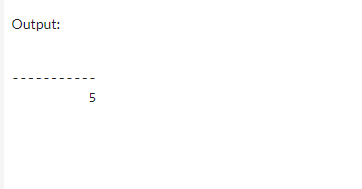
\includegraphics{./Figs/query46.png}
\end{frame}

\begin{frame}{Shtimi i Klauzolës WHERE}
\phantomsection\label{shtimi-i-klauzoluxebs-where-2}
Ju mund të shtoni një klauzolë WHERE për të specifikuar kushtet:
\end{frame}

\begin{frame}[fragile]{Shembull}
\phantomsection\label{shembull-27}
Gjeni numrin e produkteve ku çmimi është më i lartë se 20:

\AddToHookNext{env/Highlighting/begin}{\tiny}

\begin{Shaded}
\begin{Highlighting}[]
\KeywordTok{SELECT} \FunctionTok{COUNT}\NormalTok{(ProduktID)}
\KeywordTok{FROM}\NormalTok{ Produkte}
\KeywordTok{WHERE}\NormalTok{ Çmimi }\OperatorTok{\textgreater{}} \DecValTok{20}\NormalTok{;}
\end{Highlighting}
\end{Shaded}
\end{frame}

\begin{frame}{Shembull}
\phantomsection\label{shembull-28}
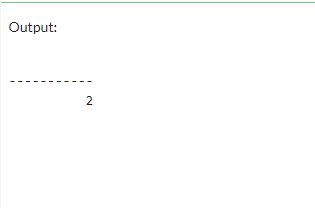
\includegraphics{./Figs/query47.png} \#\# Injoroni Dublikatat

\begin{itemize}
\item
  Ju mund të injoroni dublikatat duke përdorur fjalën kyçe DISTINCT në
  funksionin COUNT().
\item
  Nëse specifikohet DISTINCT, rreshtat me të njëjtën vlerë për kolonën e
  specifikuar do të numërohen si një.
\end{itemize}
\end{frame}

\begin{frame}[fragile]{Shembull}
\phantomsection\label{shembull-29}
Sa çmime të ndryshme ka në tabelën Produkte:

\AddToHookNext{env/Highlighting/begin}{\tiny}

\begin{Shaded}
\begin{Highlighting}[]
\KeywordTok{SELECT} \FunctionTok{COUNT}\NormalTok{(}\KeywordTok{DISTINCT}\NormalTok{ Çmimi)}
\KeywordTok{FROM}\NormalTok{ Produkte;}
\end{Highlighting}
\end{Shaded}
\end{frame}

\begin{frame}{Shembull}
\phantomsection\label{shembull-30}
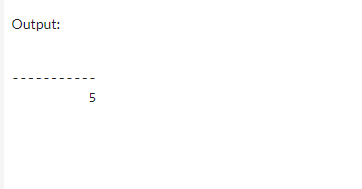
\includegraphics{./Figs/query46.png}
\end{frame}

\begin{frame}{Përdorimi i Një Alias}
\phantomsection\label{puxebrdorimi-i-njuxeb-alias}
Jepni kolonës së numëruar një emër duke përdorur fjalën kyçe AS.
\end{frame}

\begin{frame}[fragile]{Shembull}
\phantomsection\label{shembull-31}
Jepni kolonës emrin ``Numri i Rekordeve'':

\AddToHookNext{env/Highlighting/begin}{\tiny}

\begin{Shaded}
\begin{Highlighting}[]
\KeywordTok{SELECT} \FunctionTok{COUNT}\NormalTok{(}\OperatorTok{*}\NormalTok{) }\KeywordTok{AS}\NormalTok{ [Numri i Rekordeve]}
\KeywordTok{FROM}\NormalTok{ Produkte;}
\end{Highlighting}
\end{Shaded}
\end{frame}

\begin{frame}{Shembull}
\phantomsection\label{shembull-32}
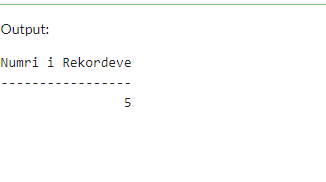
\includegraphics{./Figs/query48.png}
\end{frame}

\begin{frame}{Përdorni COUNT() me GROUP BY}
\phantomsection\label{puxebrdorni-count-me-group-by}
\begin{itemize}
\tightlist
\item
  Këtu përdorim funksionin COUNT() dhe klauzolën GROUP BY, për të kthyer
  numrin e rekordeve për secilën kategori në tabelën Produkte:
\end{itemize}
\end{frame}

\begin{frame}[fragile]{Shembull}
\phantomsection\label{shembull-33}
\AddToHookNext{env/Highlighting/begin}{\tiny}

\begin{Shaded}
\begin{Highlighting}[]
\KeywordTok{SELECT} \FunctionTok{COUNT}\NormalTok{(}\OperatorTok{*}\NormalTok{) }\KeywordTok{AS}\NormalTok{ [Numri i Rekordeve], KategoriaID}
\KeywordTok{FROM}\NormalTok{ Produkte}
\KeywordTok{GROUP} \KeywordTok{BY}\NormalTok{ KategoriaID;}
\end{Highlighting}
\end{Shaded}
\end{frame}

\begin{frame}{Shembull}
\phantomsection\label{shembull-34}
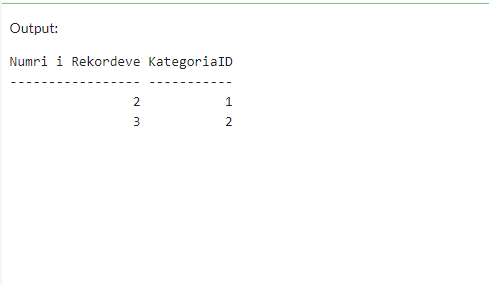
\includegraphics{./Figs/query49.png}
\end{frame}

\begin{frame}[fragile]{Funksioni SQL SUM()}
\phantomsection\label{funksioni-sql-sum}
Funksioni \texttt{SUM()} kthen shumën totale të një kolone numerike.
\end{frame}

\begin{frame}[fragile]{Tabela}
\phantomsection\label{tabela-4}
\AddToHookNext{env/Highlighting/begin}{\tiny}

\begin{Shaded}
\begin{Highlighting}[]
\CommentTok{{-}{-} Krijo tabelën DetajetPorosi}
\KeywordTok{CREATE} \KeywordTok{TABLE}\NormalTok{ DetajetPorosi (}
\NormalTok{  DetajetPorosiID }\DataTypeTok{int} \KeywordTok{PRIMARY} \KeywordTok{KEY}\NormalTok{ IDENTITY(}\DecValTok{1}\NormalTok{,}\DecValTok{1}\NormalTok{),}
\NormalTok{  PorosiaID }\DataTypeTok{int} \KeywordTok{NOT} \KeywordTok{NULL}\NormalTok{,}
\NormalTok{  ProduktiID }\DataTypeTok{int} \KeywordTok{NOT} \KeywordTok{NULL}\NormalTok{,}
\NormalTok{  Sasia }\DataTypeTok{int} \KeywordTok{NOT} \KeywordTok{NULL}
\NormalTok{);}
\end{Highlighting}
\end{Shaded}
\end{frame}

\begin{frame}[fragile]{Tabela}
\phantomsection\label{tabela-5}
\AddToHookNext{env/Highlighting/begin}{\tiny}

\begin{Shaded}
\begin{Highlighting}[]
\CommentTok{{-}{-} Mbush tabelën DetajetPorosi me të dhëna shembull}
\KeywordTok{INSERT} \KeywordTok{INTO}\NormalTok{ DetajetPorosi (PorosiaID, ProduktiID, Sasia)}
\KeywordTok{VALUES} 
\NormalTok{(}\DecValTok{10248}\NormalTok{, }\DecValTok{11}\NormalTok{, }\DecValTok{12}\NormalTok{),}
\NormalTok{(}\DecValTok{10248}\NormalTok{, }\DecValTok{42}\NormalTok{, }\DecValTok{10}\NormalTok{),}
\NormalTok{(}\DecValTok{10248}\NormalTok{, }\DecValTok{72}\NormalTok{, }\DecValTok{5}\NormalTok{),}
\NormalTok{(}\DecValTok{10249}\NormalTok{, }\DecValTok{14}\NormalTok{, }\DecValTok{9}\NormalTok{),}
\NormalTok{(}\DecValTok{10249}\NormalTok{, }\DecValTok{51}\NormalTok{, }\DecValTok{40}\NormalTok{);}
\end{Highlighting}
\end{Shaded}
\end{frame}

\begin{frame}[fragile]{Shembull}
\phantomsection\label{shembull-35}
Ktheni shumën e të gjitha fushave \texttt{Sasia} në tabelën
\texttt{DetajetPorosi}:

\AddToHookNext{env/Highlighting/begin}{\tiny}

\begin{Shaded}
\begin{Highlighting}[]
\KeywordTok{SELECT} \FunctionTok{SUM}\NormalTok{(Sasia)}
\KeywordTok{FROM}\NormalTok{ DetajetPorosi;}
\end{Highlighting}
\end{Shaded}
\end{frame}

\begin{frame}{Shembull}
\phantomsection\label{shembull-36}
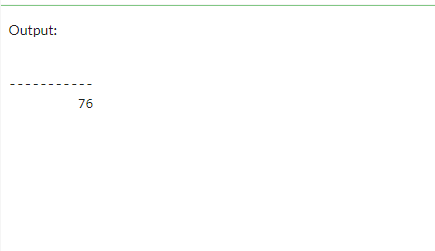
\includegraphics{./Figs/query50.png}
\end{frame}

\begin{frame}[fragile]{Sintaksa}
\phantomsection\label{sintaksa-1}
\AddToHookNext{env/Highlighting/begin}{\tiny}

\begin{Shaded}
\begin{Highlighting}[]
\KeywordTok{SELECT} \FunctionTok{SUM}\NormalTok{(emri\_i\_kolonës)}
\KeywordTok{FROM}\NormalTok{ emri\_i\_tabelës}
\KeywordTok{WHERE}\NormalTok{ kushti;}
\end{Highlighting}
\end{Shaded}
\end{frame}

\begin{frame}{Shtimi i Klauzolës WHERE}
\phantomsection\label{shtimi-i-klauzoluxebs-where-3}
Ju mund të shtoni një klauzolë WHERE për të specifikuar kushtet:
\end{frame}

\begin{frame}[fragile]{Shembull}
\phantomsection\label{shembull-37}
Ktheni shumën e fushës Sasia për produktin me ProduktiID 11:

\AddToHookNext{env/Highlighting/begin}{\tiny}

\begin{Shaded}
\begin{Highlighting}[]
\KeywordTok{SELECT} \FunctionTok{SUM}\NormalTok{(Sasia)}
\KeywordTok{FROM}\NormalTok{ DetajetPorosi}
\KeywordTok{WHERE}\NormalTok{ ProduktiID }\OperatorTok{=} \DecValTok{11}\NormalTok{;}
\end{Highlighting}
\end{Shaded}
\end{frame}

\begin{frame}{Shembull}
\phantomsection\label{shembull-38}
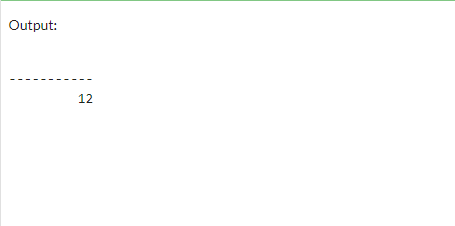
\includegraphics{./Figs/query51.png}
\end{frame}

\begin{frame}{Përdorimi i Një Alias}
\phantomsection\label{puxebrdorimi-i-njuxeb-alias-1}
Jepni kolonës së përmbledhur një emër duke përdorur fjalën kyçe AS.
\end{frame}

\begin{frame}[fragile]{Shembull}
\phantomsection\label{shembull-39}
Jepni kolonës emrin ``totali'':

\AddToHookNext{env/Highlighting/begin}{\tiny}

\begin{Shaded}
\begin{Highlighting}[]
\KeywordTok{SELECT} \FunctionTok{SUM}\NormalTok{(Sasia) }\KeywordTok{AS}\NormalTok{ totali}
\KeywordTok{FROM}\NormalTok{ DetajetPorosi;}
\end{Highlighting}
\end{Shaded}
\end{frame}

\begin{frame}{Shembull}
\phantomsection\label{shembull-40}
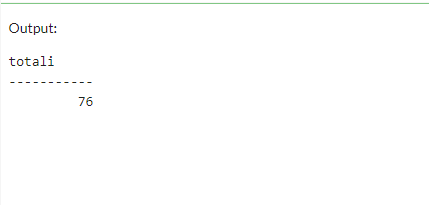
\includegraphics{./Figs/query52.png}
\end{frame}

\begin{frame}{Përdorni SUM() me GROUP BY}
\phantomsection\label{puxebrdorni-sum-me-group-by}
Këtu përdorim funksionin SUM() dhe klauzolën GROUP BY, për të kthyer
shumën e Sasia për secilin PorosiaID në tabelën DetajetPorosi:
\end{frame}

\begin{frame}[fragile]{Shembull}
\phantomsection\label{shembull-41}
\AddToHookNext{env/Highlighting/begin}{\tiny}

\begin{Shaded}
\begin{Highlighting}[]
\KeywordTok{SELECT}\NormalTok{ PorosiaID, }\FunctionTok{SUM}\NormalTok{(Sasia) }\KeywordTok{AS}\NormalTok{ [Sasia Totale]}
\KeywordTok{FROM}\NormalTok{ DetajetPorosi}
\KeywordTok{GROUP} \KeywordTok{BY}\NormalTok{ PorosiaID;}
\end{Highlighting}
\end{Shaded}
\end{frame}

\begin{frame}{Shembull}
\phantomsection\label{shembull-42}
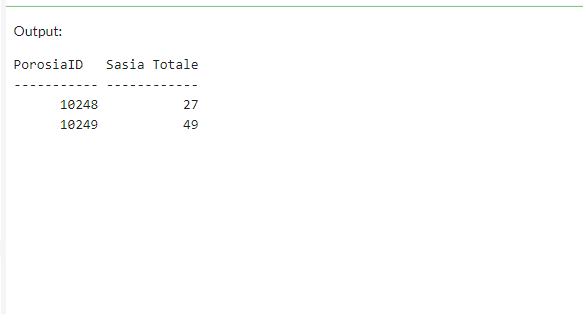
\includegraphics{./Figs/query53.png}
\end{frame}

\begin{frame}{SUM() me Një Shprehje}
\phantomsection\label{sum-me-njuxeb-shprehje}
\begin{itemize}
\item
  Parametri brenda funksionit SUM() mund të jetë gjithashtu një
  shprehje.
\item
  Nëse supozojmë se secili produkt në tabelën DetajetPorosi kushton 10
  dollarë, mund të gjejmë fitimet totale në dollarë duke shumëzuar çdo
  sasi me 10:
\end{itemize}
\end{frame}

\begin{frame}[fragile]{Shembull}
\phantomsection\label{shembull-43}
Përdorni një shprehje brenda funksionit SUM():

\AddToHookNext{env/Highlighting/begin}{\tiny}

\begin{Shaded}
\begin{Highlighting}[]
\KeywordTok{SELECT} \FunctionTok{SUM}\NormalTok{(Sasia }\OperatorTok{*} \DecValTok{10}\NormalTok{)}
\KeywordTok{FROM}\NormalTok{ DetajetPorosi;}
\end{Highlighting}
\end{Shaded}
\end{frame}

\begin{frame}{Shembull}
\phantomsection\label{shembull-44}
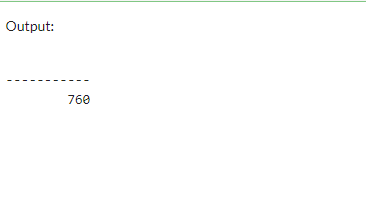
\includegraphics{./Figs/query54.png}
\end{frame}

\begin{frame}{SUM() me Një Shprehje}
\phantomsection\label{sum-me-njuxeb-shprehje-1}
Ne gjithashtu mund të bashkojmë tabelën DetajetPorosi me tabelën
Produkte për të gjetur shumën aktuale, në vend që të supozojmë se është
10 dollarë:
\end{frame}

\begin{frame}[fragile]{Tabela}
\phantomsection\label{tabela-6}
\begin{Shaded}
\begin{Highlighting}[]
\CommentTok{{-}{-} Krijo tabelën Produkte}
\KeywordTok{CREATE} \KeywordTok{TABLE}\NormalTok{ Produkte (}
\NormalTok{  ProduktiID }\DataTypeTok{int} \KeywordTok{PRIMARY} \KeywordTok{KEY}\NormalTok{ IDENTITY(}\DecValTok{1}\NormalTok{,}\DecValTok{1}\NormalTok{),}
\NormalTok{  EmriProduktit }\DataTypeTok{varchar}\NormalTok{(}\DecValTok{255}\NormalTok{) }\KeywordTok{NOT} \KeywordTok{NULL}\NormalTok{,}
\NormalTok{  Çmimi }\DataTypeTok{decimal}\NormalTok{(}\DecValTok{10}\NormalTok{, }\DecValTok{2}\NormalTok{) }\KeywordTok{NOT} \KeywordTok{NULL}
\NormalTok{);}
\end{Highlighting}
\end{Shaded}
\end{frame}

\begin{frame}[fragile]{Tabela}
\phantomsection\label{tabela-7}
\begin{Shaded}
\begin{Highlighting}[]
\CommentTok{{-}{-} Mbush tabelën Produkte me të dhëna shembull}
\KeywordTok{INSERT} \KeywordTok{INTO}\NormalTok{ Produkte (EmriProduktit, Çmimi)}
\KeywordTok{VALUES} 
\NormalTok{(}\StringTok{\textquotesingle{}Produkt1\textquotesingle{}}\NormalTok{, }\FloatTok{10.00}\NormalTok{),}
\NormalTok{(}\StringTok{\textquotesingle{}Produkt2\textquotesingle{}}\NormalTok{, }\FloatTok{20.00}\NormalTok{),}
\NormalTok{(}\StringTok{\textquotesingle{}Produkt3\textquotesingle{}}\NormalTok{, }\FloatTok{15.00}\NormalTok{);}
\end{Highlighting}
\end{Shaded}
\end{frame}

\begin{frame}[fragile]{Tabela}
\phantomsection\label{tabela-8}
\begin{Shaded}
\begin{Highlighting}[]
\CommentTok{{-}{-} Krijo tabelën DetajetPorosi}
\KeywordTok{CREATE} \KeywordTok{TABLE}\NormalTok{ DetajetPorosi (}
\NormalTok{  DetajetPorosiID }\DataTypeTok{int} \KeywordTok{PRIMARY} \KeywordTok{KEY}\NormalTok{ IDENTITY(}\DecValTok{1}\NormalTok{,}\DecValTok{1}\NormalTok{),}
\NormalTok{  PorosiaID }\DataTypeTok{int} \KeywordTok{NOT} \KeywordTok{NULL}\NormalTok{,}
\NormalTok{  ProduktiID }\DataTypeTok{int} \KeywordTok{NOT} \KeywordTok{NULL}\NormalTok{,}
\NormalTok{  Sasia }\DataTypeTok{int} \KeywordTok{NOT} \KeywordTok{NULL}
\NormalTok{);}
\end{Highlighting}
\end{Shaded}
\end{frame}

\begin{frame}[fragile]{Tabela}
\phantomsection\label{tabela-9}
\begin{Shaded}
\begin{Highlighting}[]
\CommentTok{{-}{-} Mbush tabelën DetajetPorosi me të dhëna shembull}
\KeywordTok{INSERT} \KeywordTok{INTO}\NormalTok{ DetajetPorosi (PorosiaID, ProduktiID, Sasia)}
\KeywordTok{VALUES} 
\NormalTok{(}\DecValTok{1}\NormalTok{, }\DecValTok{1}\NormalTok{, }\DecValTok{2}\NormalTok{),}
\NormalTok{(}\DecValTok{1}\NormalTok{, }\DecValTok{2}\NormalTok{, }\DecValTok{1}\NormalTok{),}
\NormalTok{(}\DecValTok{2}\NormalTok{, }\DecValTok{3}\NormalTok{, }\DecValTok{3}\NormalTok{);}
\end{Highlighting}
\end{Shaded}
\end{frame}

\begin{frame}[fragile]{Shembull}
\phantomsection\label{shembull-45}
Bashkoni tabelën DetajetPorosi me Produkte, dhe përdorni SUM() për të
gjetur shumën totale:

\AddToHookNext{env/Highlighting/begin}{\tiny}

\begin{Shaded}
\begin{Highlighting}[]
\KeywordTok{SELECT} \FunctionTok{SUM}\NormalTok{(Çmimi }\OperatorTok{*}\NormalTok{ Sasia) }\KeywordTok{AS}\NormalTok{ ShumaTotale}
\KeywordTok{FROM}\NormalTok{ DetajetPorosi}
\KeywordTok{LEFT} \KeywordTok{JOIN}\NormalTok{ Produkte }\KeywordTok{ON}\NormalTok{ DetajetPorosi.ProduktiID }\OperatorTok{=}\NormalTok{ Produkte.ProduktiID;}
\end{Highlighting}
\end{Shaded}
\end{frame}

\begin{frame}{Shembull}
\phantomsection\label{shembull-46}
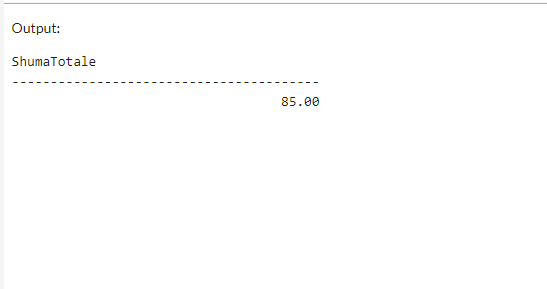
\includegraphics{./Figs/query56.png}
\end{frame}

\end{document}
